\section{Dijkstra}
\clearpage
\subsection*{Mean request latency}
\begin{center}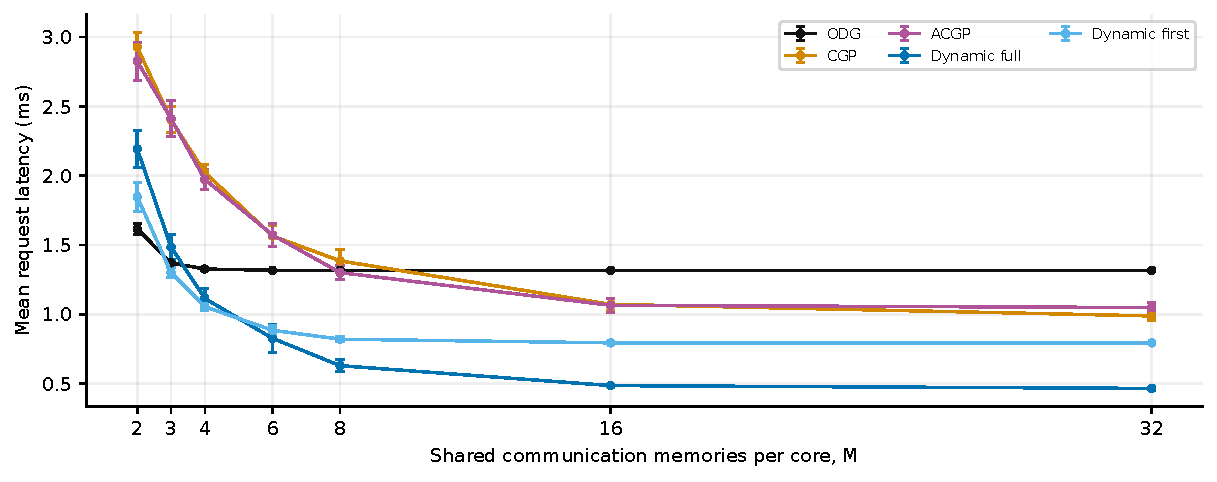
\includegraphics[width=.94\linewidth,height=.255\textheight,keepaspectratio]{figures/memory/torus_dijkstra_request_latency_mean_ms.pdf}\captionof{figure}{Run-level mean and sample SD. Shared trace aliases are counted once.}\end{center}
\begin{center}{\scriptsize\setlength{\tabcolsep}{3pt}
\begin{tabular}{lrrrrr}
\toprule
M & ODG & CGP & ACGP & Dynamic full & Dynamic first \\
\midrule
2 & $1.616\pm0.041$ & $2.927\pm0.108$ & $2.826\pm0.137$ & $2.194\pm0.131$ & $1.848\pm0.105$ \\
3 & $1.370\pm0.021$ & $2.403\pm0.094$ & $2.412\pm0.130$ & $1.484\pm0.089$ & $1.301\pm0.038$ \\
4 & $1.326\pm0.008$ & $2.022\pm0.059$ & $1.973\pm0.072$ & $1.113\pm0.073$ & $1.054\pm0.024$ \\
6 & $1.317\pm0.003$ & $1.564\pm0.074$ & $1.572\pm0.082$ & $0.8259\pm0.0993$ & $0.8837\pm0.0307$ \\
8 & $1.317\pm0.003$ & $1.385\pm0.082$ & $1.300\pm0.048$ & $0.6283\pm0.0424$ & $0.8194\pm0.0191$ \\
16 & $1.317\pm0.003$ & $1.071\pm0.041$ & $1.064\pm0.050$ & $0.4844\pm0.0056$ & $0.7930\pm0.0051$ \\
32 & $1.317\pm0.003$ & $0.9872\pm0.0292$ & $1.048\pm0.035$ & $0.4640\pm0.0023$ & $0.7928\pm0.0050$ \\
\bottomrule\end{tabular}}
\captionof{table}{Mean $\pm$ sample SD; n/a denotes a metric outside that policy's instrumentation.}
{\footnotesize\href{https://github.com/sanjeevkrishnaa/Compiler-Driven-ACE/blob/codex/ace-scheduler-correctness/docs/latex/qft96_final/data/memory_torus_dijkstra_request_latency_mean_ms.csv}{Exact CSV values and sample counts}}
\end{center}
\subsection*{Median request latency}
\begin{center}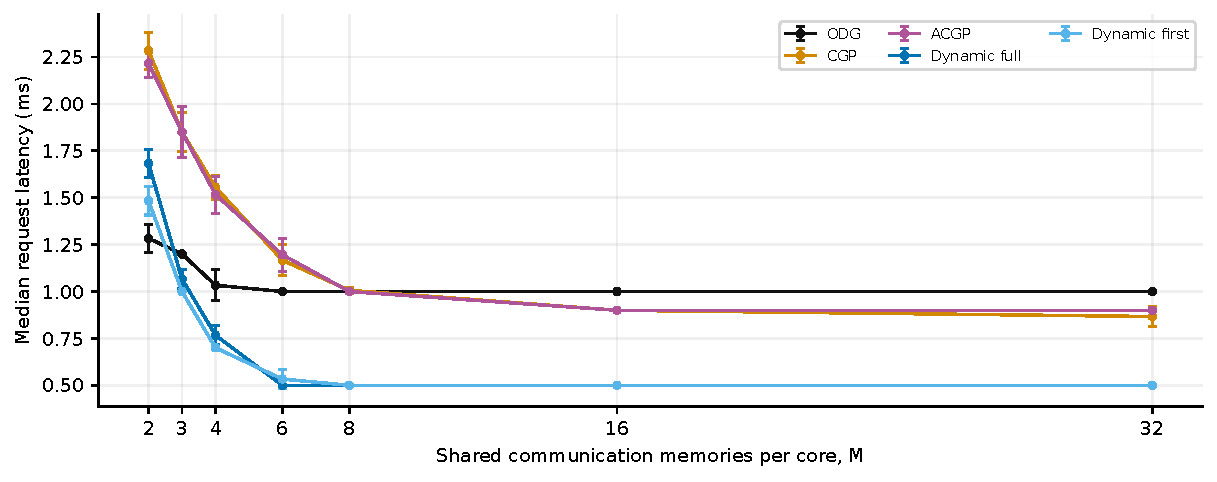
\includegraphics[width=.94\linewidth,height=.255\textheight,keepaspectratio]{figures/memory/torus_dijkstra_request_latency_median_ms.pdf}\captionof{figure}{Run-level mean and sample SD. Shared trace aliases are counted once.}\end{center}
\begin{center}{\scriptsize\setlength{\tabcolsep}{3pt}
\begin{tabular}{lrrrrr}
\toprule
M & ODG & CGP & ACGP & Dynamic full & Dynamic first \\
\midrule
2 & $1.283\pm0.075$ & $2.283\pm0.098$ & $2.217\pm0.075$ & $1.683\pm0.075$ & $1.483\pm0.075$ \\
3 & $1.200\pm0.000$ & $1.850\pm0.105$ & $1.850\pm0.138$ & $1.067\pm0.052$ & $1.000\pm0.000$ \\
4 & $1.033\pm0.082$ & $1.556\pm0.063$ & $1.517\pm0.098$ & $0.7667\pm0.0516$ & $0.7000\pm0.0000$ \\
6 & $1.000\pm0.000$ & $1.167\pm0.082$ & $1.196\pm0.088$ & $0.5000\pm0.0000$ & $0.5333\pm0.0516$ \\
8 & $1.000\pm0.000$ & $1.006\pm0.016$ & $1.000\pm0.000$ & $0.5000\pm0.0000$ & $0.5000\pm0.0000$ \\
16 & $1.000\pm0.000$ & $0.9000\pm0.0000$ & $0.9000\pm0.0000$ & $0.5000\pm0.0000$ & $0.5000\pm0.0000$ \\
32 & $1.000\pm0.000$ & $0.8667\pm0.0516$ & $0.9000\pm0.0000$ & $0.5000\pm0.0000$ & $0.5000\pm0.0000$ \\
\bottomrule\end{tabular}}
\captionof{table}{Mean $\pm$ sample SD; n/a denotes a metric outside that policy's instrumentation.}
{\footnotesize\href{https://github.com/sanjeevkrishnaa/Compiler-Driven-ACE/blob/codex/ace-scheduler-correctness/docs/latex/qft96_final/data/memory_torus_dijkstra_request_latency_median_ms.csv}{Exact CSV values and sample counts}}
\end{center}
\clearpage
\subsection*{p95 request latency}
\begin{center}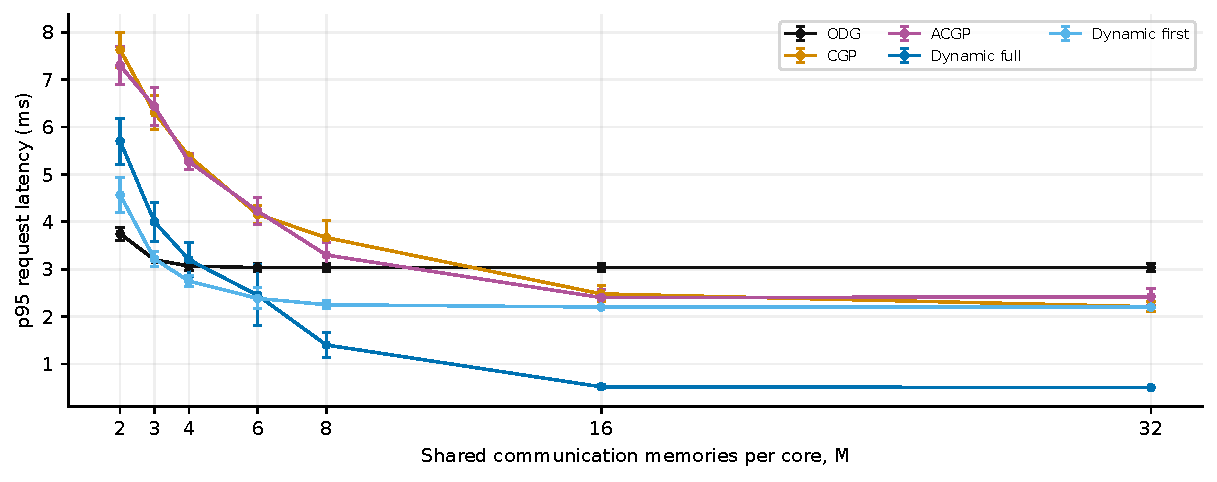
\includegraphics[width=.94\linewidth,height=.255\textheight,keepaspectratio]{figures/memory/torus_dijkstra_request_latency_p95_ms.pdf}\captionof{figure}{Run-level mean and sample SD. Shared trace aliases are counted once.}\end{center}
\begin{center}{\scriptsize\setlength{\tabcolsep}{3pt}
\begin{tabular}{lrrrrr}
\toprule
M & ODG & CGP & ACGP & Dynamic full & Dynamic first \\
\midrule
2 & $3.750\pm0.138$ & $7.634\pm0.367$ & $7.300\pm0.405$ & $5.700\pm0.482$ & $4.567\pm0.367$ \\
3 & $3.200\pm0.000$ & $6.302\pm0.357$ & $6.433\pm0.398$ & $4.000\pm0.410$ & $3.217\pm0.160$ \\
4 & $3.067\pm0.103$ & $5.388\pm0.045$ & $5.273\pm0.173$ & $3.200\pm0.363$ & $2.750\pm0.122$ \\
6 & $3.033\pm0.082$ & $4.158\pm0.185$ & $4.228\pm0.289$ & $2.450\pm0.638$ & $2.383\pm0.223$ \\
8 & $3.033\pm0.082$ & $3.667\pm0.367$ & $3.300\pm0.261$ & $1.400\pm0.261$ & $2.250\pm0.084$ \\
16 & $3.033\pm0.082$ & $2.479\pm0.169$ & $2.400\pm0.179$ & $0.5167\pm0.0408$ & $2.200\pm0.000$ \\
32 & $3.033\pm0.082$ & $2.207\pm0.107$ & $2.417\pm0.183$ & $0.5000\pm0.0000$ & $2.200\pm0.000$ \\
\bottomrule\end{tabular}}
\captionof{table}{Mean $\pm$ sample SD; n/a denotes a metric outside that policy's instrumentation.}
{\footnotesize\href{https://github.com/sanjeevkrishnaa/Compiler-Driven-ACE/blob/codex/ace-scheduler-correctness/docs/latex/qft96_final/data/memory_torus_dijkstra_request_latency_p95_ms.csv}{Exact CSV values and sample counts}}
\end{center}
\subsection*{Maximum request latency}
\begin{center}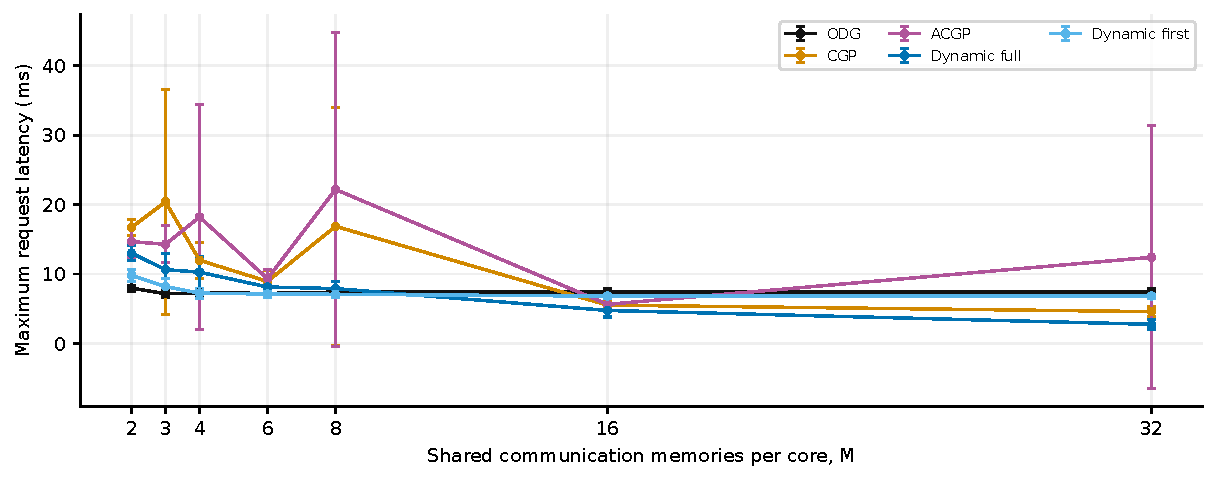
\includegraphics[width=.94\linewidth,height=.255\textheight,keepaspectratio]{figures/memory/torus_dijkstra_request_latency_max_ms.pdf}\captionof{figure}{Run-level mean and sample SD. Shared trace aliases are counted once.}\end{center}
\begin{center}{\scriptsize\setlength{\tabcolsep}{3pt}
\begin{tabular}{lrrrrr}
\toprule
M & ODG & CGP & ACGP & Dynamic full & Dynamic first \\
\midrule
2 & $7.967\pm0.418$ & $16.717\pm1.182$ & $14.666\pm2.211$ & $13.000\pm1.043$ & $9.834\pm0.859$ \\
3 & $7.150\pm0.505$ & $20.400\pm16.209$ & $14.284\pm2.676$ & $10.634\pm2.318$ & $8.184\pm1.160$ \\
4 & $7.317\pm0.376$ & $11.984\pm2.593$ & $18.200\pm16.160$ & $10.267\pm2.315$ & $7.250\pm0.718$ \\
6 & $7.200\pm0.341$ & $8.934\pm1.540$ & $9.334\pm1.271$ & $8.134\pm1.382$ & $7.117\pm0.549$ \\
8 & $7.400\pm0.510$ & $16.867\pm17.116$ & $22.179\pm22.637$ & $7.900\pm1.056$ & $7.084\pm0.440$ \\
16 & $7.400\pm0.510$ & $5.517\pm0.581$ & $5.633\pm1.815$ & $4.750\pm0.938$ & $6.817\pm0.286$ \\
32 & $7.400\pm0.510$ & $4.583\pm0.671$ & $12.408\pm18.935$ & $2.750\pm0.669$ & $6.817\pm0.286$ \\
\bottomrule\end{tabular}}
\captionof{table}{Mean $\pm$ sample SD; n/a denotes a metric outside that policy's instrumentation.}
{\footnotesize\href{https://github.com/sanjeevkrishnaa/Compiler-Driven-ACE/blob/codex/ace-scheduler-correctness/docs/latex/qft96_final/data/memory_torus_dijkstra_request_latency_max_ms.csv}{Exact CSV values and sample counts}}
\end{center}
\clearpage
\subsection*{Communication makespan}
\begin{center}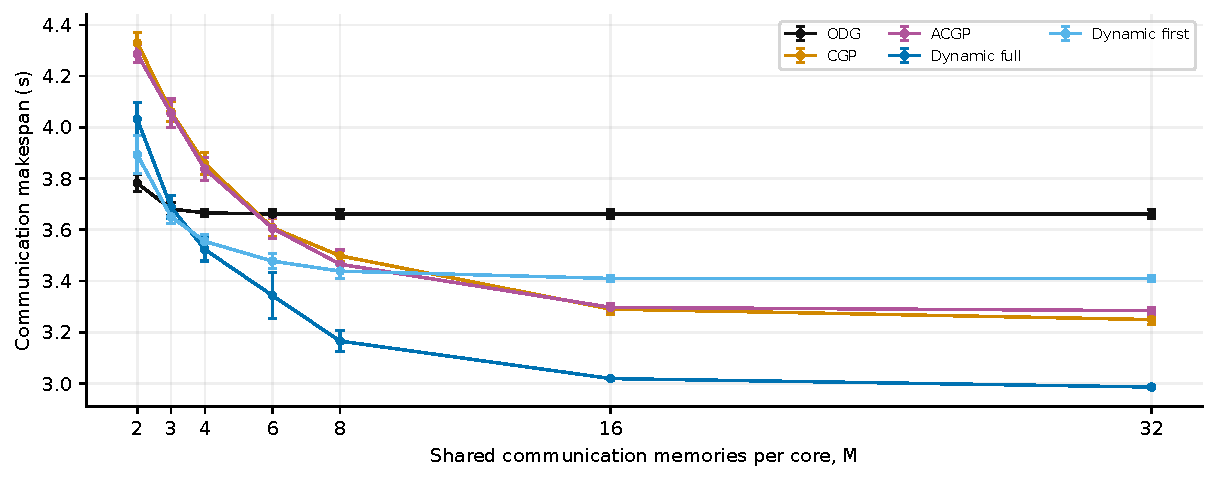
\includegraphics[width=.94\linewidth,height=.255\textheight,keepaspectratio]{figures/memory/torus_dijkstra_end_to_end_latency_ms.pdf}\captionof{figure}{Run-level mean and sample SD. Shared trace aliases are counted once.}\end{center}
\begin{center}{\scriptsize\setlength{\tabcolsep}{3pt}
\begin{tabular}{lrrrrr}
\toprule
M & ODG & CGP & ACGP & Dynamic full & Dynamic first \\
\midrule
2 & $3.782\pm0.033$ & $4.330\pm0.041$ & $4.287\pm0.035$ & $4.032\pm0.065$ & $3.894\pm0.073$ \\
3 & $3.681\pm0.026$ & $4.061\pm0.038$ & $4.055\pm0.055$ & $3.689\pm0.046$ & $3.651\pm0.025$ \\
4 & $3.666\pm0.014$ & $3.858\pm0.042$ & $3.837\pm0.046$ & $3.523\pm0.045$ & $3.555\pm0.025$ \\
6 & $3.662\pm0.016$ & $3.608\pm0.036$ & $3.606\pm0.041$ & $3.343\pm0.088$ & $3.478\pm0.030$ \\
8 & $3.662\pm0.016$ & $3.498\pm0.022$ & $3.466\pm0.055$ & $3.165\pm0.042$ & $3.439\pm0.028$ \\
16 & $3.662\pm0.016$ & $3.290\pm0.022$ & $3.297\pm0.017$ & $3.019\pm0.004$ & $3.410\pm0.011$ \\
32 & $3.662\pm0.016$ & $3.249\pm0.018$ & $3.284\pm0.014$ & $2.986\pm0.007$ & $3.409\pm0.011$ \\
\bottomrule\end{tabular}}
\captionof{table}{Mean $\pm$ sample SD; n/a denotes a metric outside that policy's instrumentation.}
{\footnotesize\href{https://github.com/sanjeevkrishnaa/Compiler-Driven-ACE/blob/codex/ace-scheduler-correctness/docs/latex/qft96_final/data/memory_torus_dijkstra_end_to_end_latency_ms.csv}{Exact CSV values and sample counts}}
\end{center}
\subsection*{Mean admission wait}
\begin{center}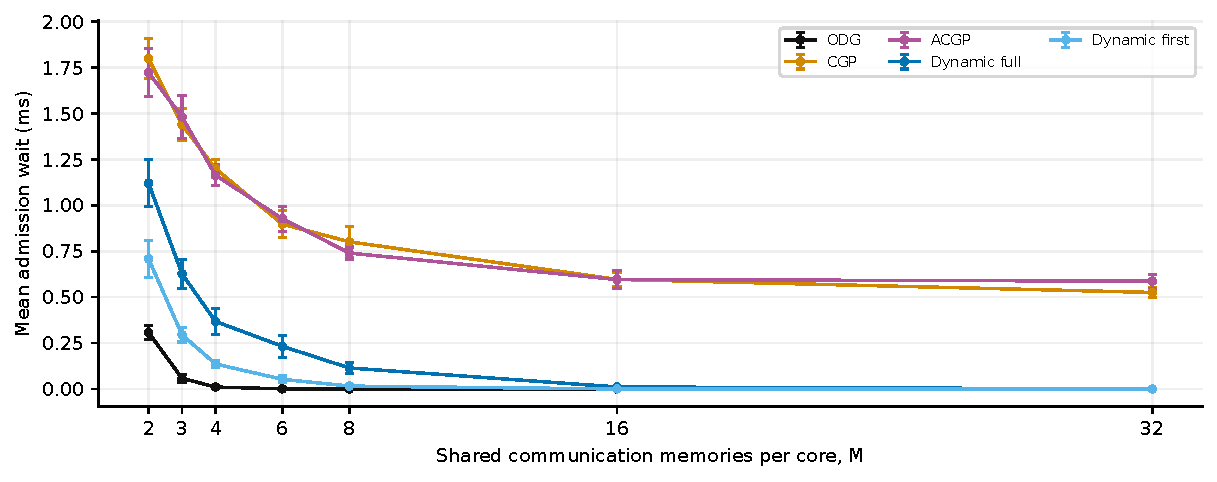
\includegraphics[width=.94\linewidth,height=.255\textheight,keepaspectratio]{figures/memory/torus_dijkstra_average_admission_wait_ms.pdf}\captionof{figure}{Run-level mean and sample SD. Shared trace aliases are counted once.}\end{center}
\begin{center}{\scriptsize\setlength{\tabcolsep}{3pt}
\begin{tabular}{lrrrrr}
\toprule
M & ODG & CGP & ACGP & Dynamic full & Dynamic first \\
\midrule
2 & $0.3075\pm0.0402$ & $1.799\pm0.110$ & $1.723\pm0.130$ & $1.120\pm0.128$ & $0.7084\pm0.1012$ \\
3 & $0.0581\pm0.0199$ & $1.439\pm0.086$ & $1.481\pm0.116$ & $0.6267\pm0.0805$ & $0.2952\pm0.0394$ \\
4 & $0.0106\pm0.0073$ & $1.199\pm0.048$ & $1.164\pm0.057$ & $0.3678\pm0.0718$ & $0.1362\pm0.0187$ \\
6 & $0.0006\pm0.0007$ & $0.8976\pm0.0744$ & $0.9266\pm0.0688$ & $0.2324\pm0.0600$ & $0.0527\pm0.0183$ \\
8 & $0.0000\pm0.0000$ & $0.8013\pm0.0835$ & $0.7403\pm0.0326$ & $0.1146\pm0.0318$ & $0.0158\pm0.0079$ \\
16 & $0.0000\pm0.0000$ & $0.5967\pm0.0364$ & $0.5956\pm0.0475$ & $0.0111\pm0.0048$ & $0.0001\pm0.0002$ \\
32 & $0.0000\pm0.0000$ & $0.5255\pm0.0278$ & $0.5871\pm0.0382$ & $0.0001\pm0.0004$ & $0.0000\pm0.0000$ \\
\bottomrule\end{tabular}}
\captionof{table}{Mean $\pm$ sample SD; n/a denotes a metric outside that policy's instrumentation.}
{\footnotesize\href{https://github.com/sanjeevkrishnaa/Compiler-Driven-ACE/blob/codex/ace-scheduler-correctness/docs/latex/qft96_final/data/memory_torus_dijkstra_average_admission_wait_ms.csv}{Exact CSV values and sample counts}}
\end{center}
\clearpage
\subsection*{Delivered EPR fidelity}
\begin{center}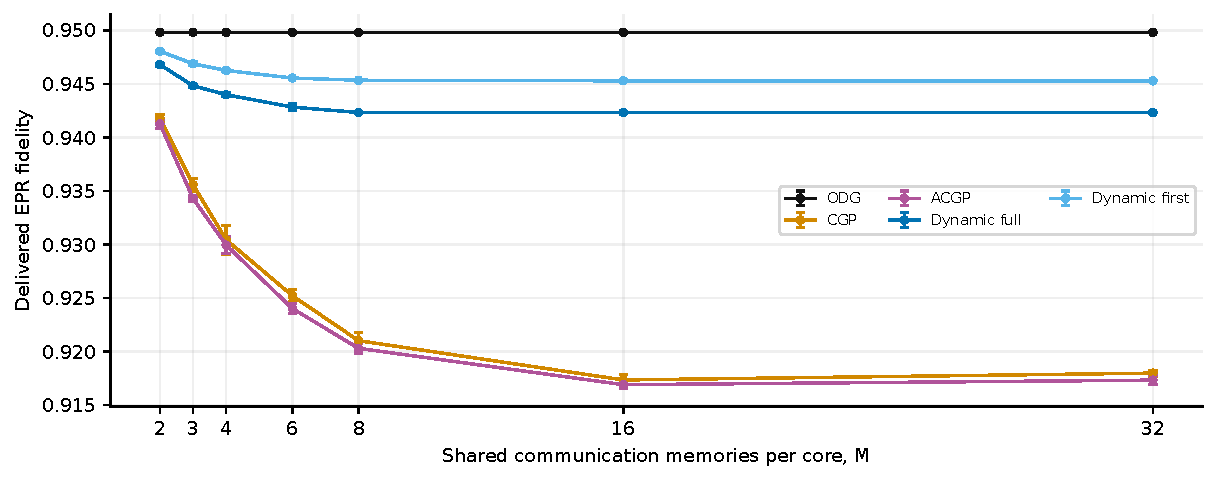
\includegraphics[width=.94\linewidth,height=.255\textheight,keepaspectratio]{figures/memory/torus_dijkstra_average_delivered_epr_fidelity.pdf}\captionof{figure}{Run-level mean and sample SD. Shared trace aliases are counted once.}\end{center}
\begin{center}{\scriptsize\setlength{\tabcolsep}{3pt}
\begin{tabular}{lrrrrr}
\toprule
M & ODG & CGP & ACGP & Dynamic full & Dynamic first \\
\midrule
2 & $0.9498\pm0.0000$ & $0.9418\pm0.0003$ & $0.9413\pm0.0004$ & $0.9468\pm0.0001$ & $0.9480\pm0.0001$ \\
3 & $0.9498\pm0.0000$ & $0.9356\pm0.0006$ & $0.9343\pm0.0003$ & $0.9448\pm0.0001$ & $0.9469\pm0.0002$ \\
4 & $0.9498\pm0.0000$ & $0.9304\pm0.0013$ & $0.9299\pm0.0008$ & $0.9440\pm0.0002$ & $0.9463\pm0.0001$ \\
6 & $0.9498\pm0.0000$ & $0.9252\pm0.0005$ & $0.9240\pm0.0005$ & $0.9428\pm0.0004$ & $0.9455\pm0.0001$ \\
8 & $0.9498\pm0.0000$ & $0.9210\pm0.0008$ & $0.9203\pm0.0004$ & $0.9423\pm0.0000$ & $0.9453\pm0.0000$ \\
16 & $0.9498\pm0.0000$ & $0.9173\pm0.0005$ & $0.9169\pm0.0004$ & $0.9423\pm0.0000$ & $0.9453\pm0.0000$ \\
32 & $0.9498\pm0.0000$ & $0.9180\pm0.0003$ & $0.9173\pm0.0004$ & $0.9423\pm0.0000$ & $0.9453\pm0.0000$ \\
\bottomrule\end{tabular}}
\captionof{table}{Mean $\pm$ sample SD; n/a denotes a metric outside that policy's instrumentation.}
{\footnotesize\href{https://github.com/sanjeevkrishnaa/Compiler-Driven-ACE/blob/codex/ace-scheduler-correctness/docs/latex/qft96_final/data/memory_torus_dijkstra_average_delivered_epr_fidelity.csv}{Exact CSV values and sample counts}}
\end{center}
\subsection*{Compiler readiness fraction}
\begin{center}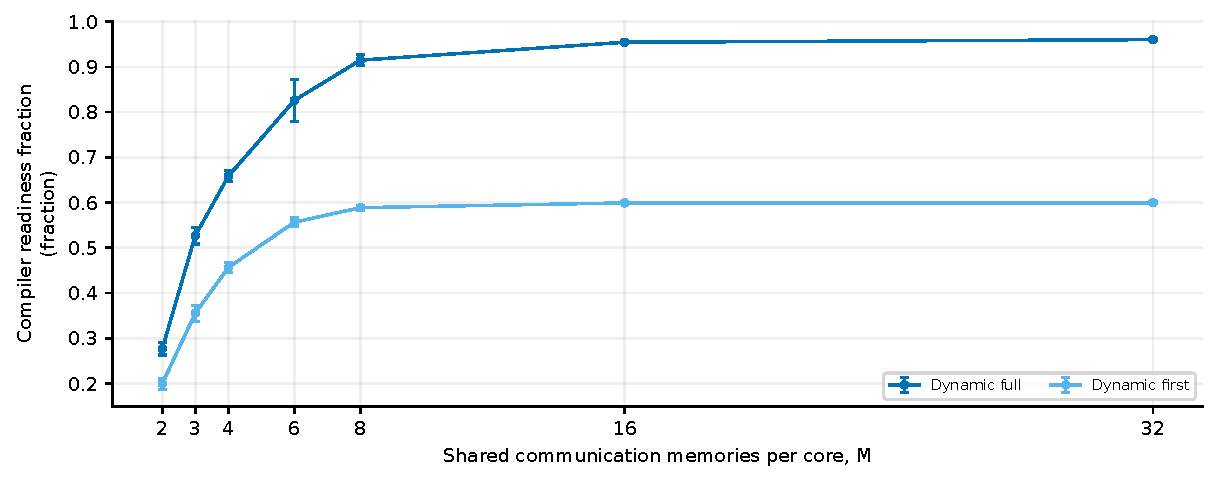
\includegraphics[width=.94\linewidth,height=.255\textheight,keepaspectratio]{figures/memory/torus_dijkstra_pregenerated_success_rate.pdf}\captionof{figure}{Run-level mean and sample SD. Shared trace aliases are counted once.}\end{center}
\begin{center}{\scriptsize\setlength{\tabcolsep}{3pt}
\begin{tabular}{lrrrrr}
\toprule
M & ODG & CGP & ACGP & Dynamic full & Dynamic first \\
\midrule
2 & n/a & n/a & n/a & $0.2766\pm0.0138$ & $0.1997\pm0.0122$ \\
3 & n/a & n/a & n/a & $0.5266\pm0.0184$ & $0.3553\pm0.0179$ \\
4 & n/a & n/a & n/a & $0.6581\pm0.0120$ & $0.4562\pm0.0116$ \\
6 & n/a & n/a & n/a & $0.8258\pm0.0462$ & $0.5565\pm0.0094$ \\
8 & n/a & n/a & n/a & $0.9148\pm0.0124$ & $0.5886\pm0.0057$ \\
16 & n/a & n/a & n/a & $0.9544\pm0.0032$ & $0.5992\pm0.0017$ \\
32 & n/a & n/a & n/a & $0.9602\pm0.0025$ & $0.5993\pm0.0017$ \\
\bottomrule\end{tabular}}
\captionof{table}{Mean $\pm$ sample SD; n/a denotes a metric outside that policy's instrumentation.}
{\footnotesize\href{https://github.com/sanjeevkrishnaa/Compiler-Driven-ACE/blob/codex/ace-scheduler-correctness/docs/latex/qft96_final/data/memory_torus_dijkstra_pregenerated_success_rate.csv}{Exact CSV values and sample counts}}
\end{center}
\clearpage
\subsection*{Intended compiler-hit fraction}
\begin{center}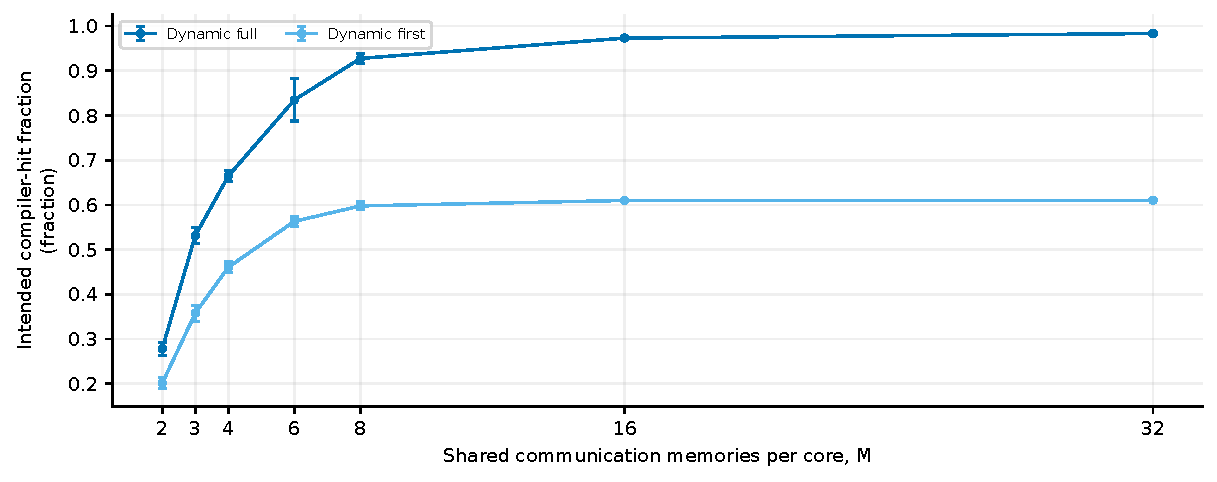
\includegraphics[width=.94\linewidth,height=.255\textheight,keepaspectratio]{figures/memory/torus_dijkstra_intended_request_hit_rate.pdf}\captionof{figure}{Run-level mean and sample SD. Shared trace aliases are counted once.}\end{center}
\begin{center}{\scriptsize\setlength{\tabcolsep}{3pt}
\begin{tabular}{lrrrrr}
\toprule
M & ODG & CGP & ACGP & Dynamic full & Dynamic first \\
\midrule
2 & n/a & n/a & n/a & $0.2782\pm0.0143$ & $0.2012\pm0.0125$ \\
3 & n/a & n/a & n/a & $0.5313\pm0.0180$ & $0.3578\pm0.0180$ \\
4 & n/a & n/a & n/a & $0.6646\pm0.0114$ & $0.4606\pm0.0117$ \\
6 & n/a & n/a & n/a & $0.8349\pm0.0471$ & $0.5632\pm0.0113$ \\
8 & n/a & n/a & n/a & $0.9277\pm0.0110$ & $0.5977\pm0.0087$ \\
16 & n/a & n/a & n/a & $0.9733\pm0.0038$ & $0.6100\pm0.0012$ \\
32 & n/a & n/a & n/a & $0.9835\pm0.0026$ & $0.6104\pm0.0008$ \\
\bottomrule\end{tabular}}
\captionof{table}{Mean $\pm$ sample SD; n/a denotes a metric outside that policy's instrumentation.}
{\footnotesize\href{https://github.com/sanjeevkrishnaa/Compiler-Driven-ACE/blob/codex/ace-scheduler-correctness/docs/latex/qft96_final/data/memory_torus_dijkstra_intended_request_hit_rate.csv}{Exact CSV values and sample counts}}
\end{center}
\subsection*{Compiler fallback fraction}
\begin{center}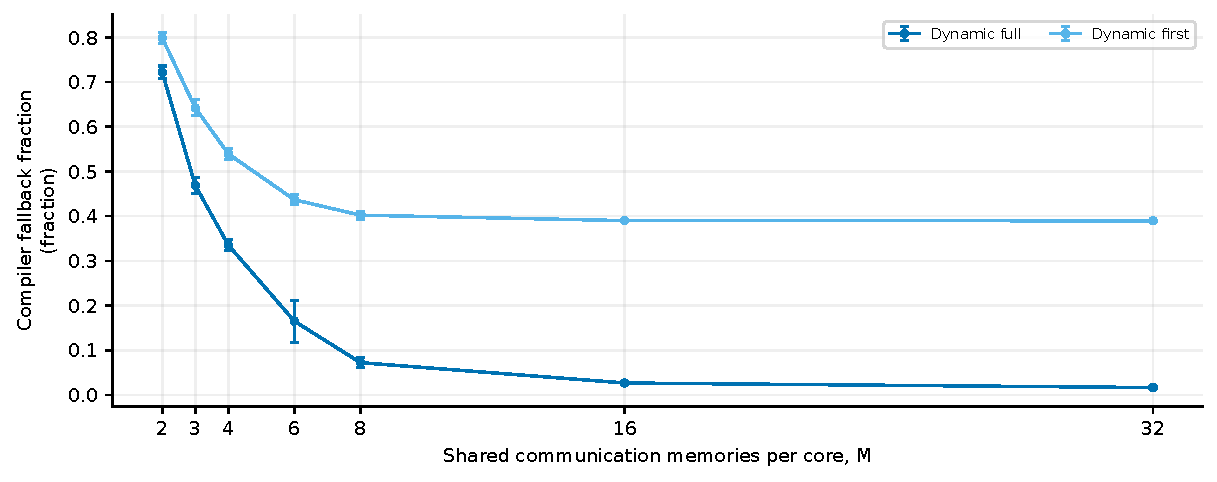
\includegraphics[width=.94\linewidth,height=.255\textheight,keepaspectratio]{figures/memory/torus_dijkstra_on_demand_fallback_rate.pdf}\captionof{figure}{Run-level mean and sample SD. Shared trace aliases are counted once.}\end{center}
\begin{center}{\scriptsize\setlength{\tabcolsep}{3pt}
\begin{tabular}{lrrrrr}
\toprule
M & ODG & CGP & ACGP & Dynamic full & Dynamic first \\
\midrule
2 & n/a & n/a & n/a & $0.7218\pm0.0143$ & $0.7988\pm0.0125$ \\
3 & n/a & n/a & n/a & $0.4687\pm0.0180$ & $0.6422\pm0.0180$ \\
4 & n/a & n/a & n/a & $0.3354\pm0.0114$ & $0.5394\pm0.0117$ \\
6 & n/a & n/a & n/a & $0.1651\pm0.0471$ & $0.4368\pm0.0113$ \\
8 & n/a & n/a & n/a & $0.0723\pm0.0110$ & $0.4023\pm0.0087$ \\
16 & n/a & n/a & n/a & $0.0267\pm0.0038$ & $0.3900\pm0.0012$ \\
32 & n/a & n/a & n/a & $0.0165\pm0.0026$ & $0.3896\pm0.0008$ \\
\bottomrule\end{tabular}}
\captionof{table}{Mean $\pm$ sample SD; n/a denotes a metric outside that policy's instrumentation.}
{\footnotesize\href{https://github.com/sanjeevkrishnaa/Compiler-Driven-ACE/blob/codex/ace-scheduler-correctness/docs/latex/qft96_final/data/memory_torus_dijkstra_on_demand_fallback_rate.csv}{Exact CSV values and sample counts}}
\end{center}
\clearpage
\subsection*{Compiler-cache waste}
\begin{center}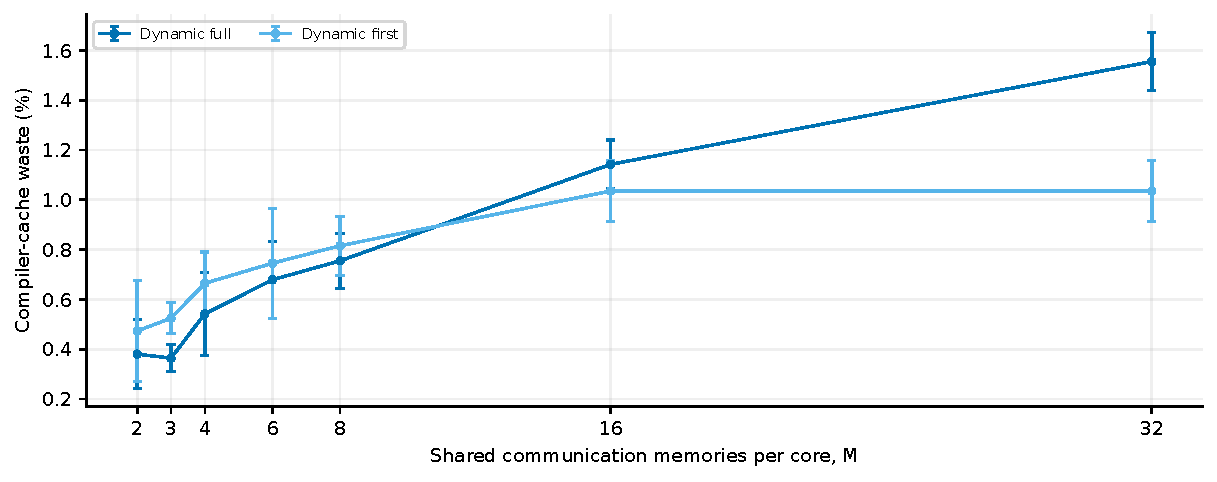
\includegraphics[width=.94\linewidth,height=.255\textheight,keepaspectratio]{figures/memory/torus_dijkstra_compiler_waste_percentage.pdf}\captionof{figure}{Run-level mean and sample SD. Shared trace aliases are counted once.}\end{center}
\begin{center}{\scriptsize\setlength{\tabcolsep}{3pt}
\begin{tabular}{lrrrrr}
\toprule
M & ODG & CGP & ACGP & Dynamic full & Dynamic first \\
\midrule
2 & n/a & n/a & n/a & $0.3802\pm0.1390$ & $0.4732\pm0.2043$ \\
3 & n/a & n/a & n/a & $0.3642\pm0.0530$ & $0.5246\pm0.0614$ \\
4 & n/a & n/a & n/a & $0.5420\pm0.1678$ & $0.6647\pm0.1258$ \\
6 & n/a & n/a & n/a & $0.6789\pm0.1544$ & $0.7455\pm0.2207$ \\
8 & n/a & n/a & n/a & $0.7550\pm0.1098$ & $0.8155\pm0.1181$ \\
16 & n/a & n/a & n/a & $1.142\pm0.098$ & $1.035\pm0.123$ \\
32 & n/a & n/a & n/a & $1.555\pm0.117$ & $1.035\pm0.123$ \\
\bottomrule\end{tabular}}
\captionof{table}{Mean $\pm$ sample SD; n/a denotes a metric outside that policy's instrumentation.}
{\footnotesize\href{https://github.com/sanjeevkrishnaa/Compiler-Driven-ACE/blob/codex/ace-scheduler-correctness/docs/latex/qft96_final/data/memory_torus_dijkstra_compiler_waste_percentage.csv}{Exact CSV values and sample counts}}
\end{center}
\subsection*{Native-protocol waste}
\begin{center}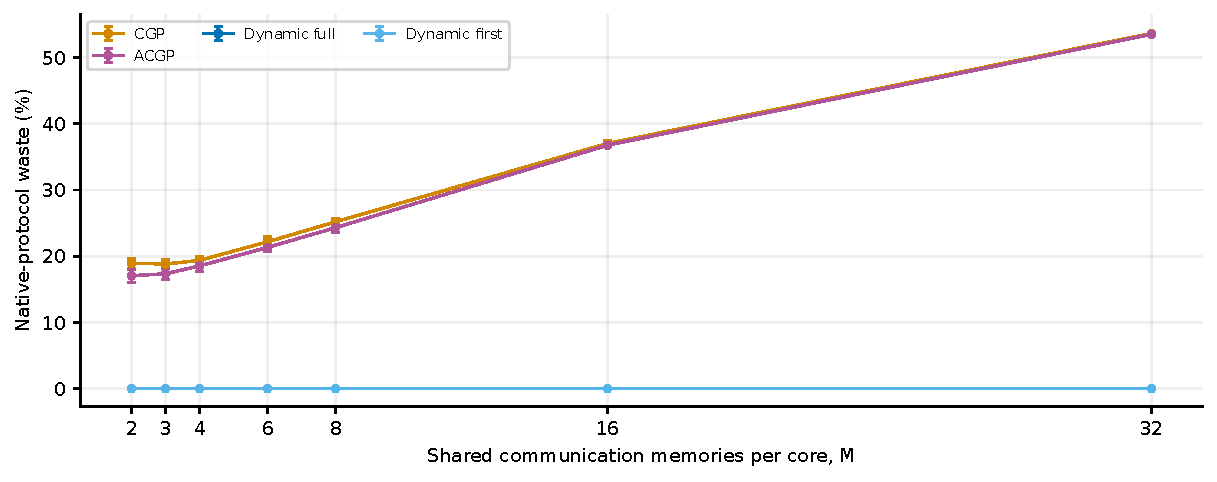
\includegraphics[width=.94\linewidth,height=.255\textheight,keepaspectratio]{figures/memory/torus_dijkstra_protocol_waste_percentage.pdf}\captionof{figure}{Run-level mean and sample SD. Shared trace aliases are counted once.}\end{center}
\begin{center}{\scriptsize\setlength{\tabcolsep}{3pt}
\begin{tabular}{lrrrrr}
\toprule
M & ODG & CGP & ACGP & Dynamic full & Dynamic first \\
\midrule
2 & n/a & $18.968\pm0.748$ & $17.064\pm1.004$ & $0.0000\pm0.0000$ & $0.0000\pm0.0000$ \\
3 & n/a & $18.830\pm0.635$ & $17.361\pm0.872$ & $0.0000\pm0.0000$ & $0.0000\pm0.0000$ \\
4 & n/a & $19.381\pm0.582$ & $18.545\pm0.873$ & $0.0000\pm0.0000$ & $0.0000\pm0.0000$ \\
6 & n/a & $22.186\pm0.725$ & $21.339\pm0.651$ & $0.0000\pm0.0000$ & $0.0000\pm0.0000$ \\
8 & n/a & $25.199\pm0.444$ & $24.321\pm0.795$ & $0.0000\pm0.0000$ & $0.0000\pm0.0000$ \\
16 & n/a & $37.033\pm0.412$ & $36.773\pm0.158$ & $0.0000\pm0.0000$ & $0.0000\pm0.0000$ \\
32 & n/a & $53.657\pm0.159$ & $53.528\pm0.075$ & $0.0000\pm0.0000$ & $0.0000\pm0.0000$ \\
\bottomrule\end{tabular}}
\captionof{table}{Mean $\pm$ sample SD; n/a denotes a metric outside that policy's instrumentation.}
{\footnotesize\href{https://github.com/sanjeevkrishnaa/Compiler-Driven-ACE/blob/codex/ace-scheduler-correctness/docs/latex/qft96_final/data/memory_torus_dijkstra_protocol_waste_percentage.csv}{Exact CSV values and sample counts}}
\end{center}
\clearpage
\subsection*{Compiler-pair expiry}
\begin{center}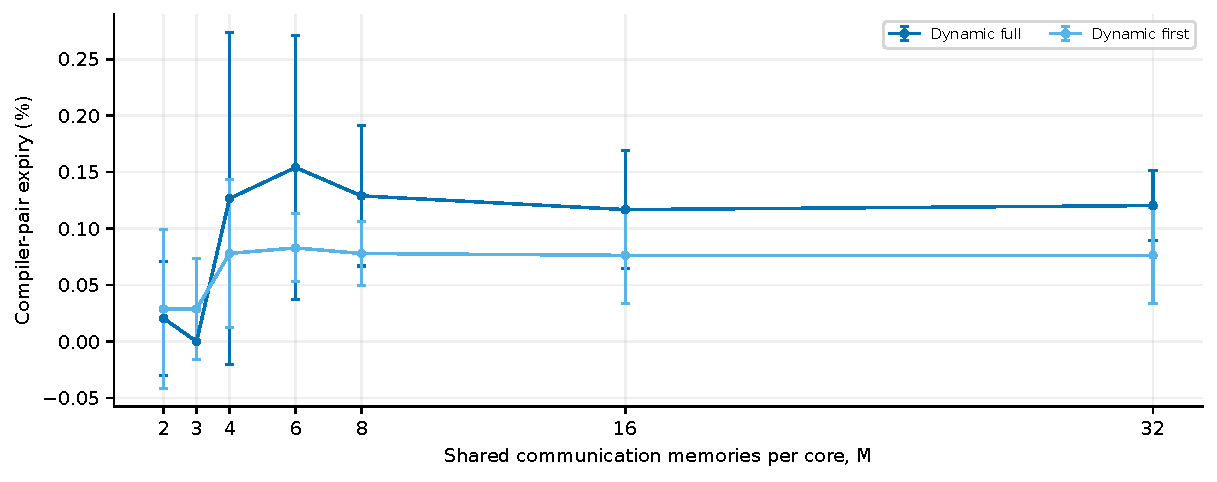
\includegraphics[width=.94\linewidth,height=.255\textheight,keepaspectratio]{figures/memory/torus_dijkstra_compiler_expiry_percentage.pdf}\captionof{figure}{Run-level mean and sample SD. Shared trace aliases are counted once.}\end{center}
\begin{center}{\scriptsize\setlength{\tabcolsep}{3pt}
\begin{tabular}{lrrrrr}
\toprule
M & ODG & CGP & ACGP & Dynamic full & Dynamic first \\
\midrule
2 & n/a & n/a & n/a & $0.0206\pm0.0505$ & $0.0288\pm0.0706$ \\
3 & n/a & n/a & n/a & $0.0000\pm0.0000$ & $0.0288\pm0.0447$ \\
4 & n/a & n/a & n/a & $0.1267\pm0.1472$ & $0.0780\pm0.0657$ \\
6 & n/a & n/a & n/a & $0.1541\pm0.1167$ & $0.0829\pm0.0301$ \\
8 & n/a & n/a & n/a & $0.1290\pm0.0621$ & $0.0780\pm0.0280$ \\
16 & n/a & n/a & n/a & $0.1169\pm0.0520$ & $0.0763\pm0.0426$ \\
32 & n/a & n/a & n/a & $0.1204\pm0.0309$ & $0.0763\pm0.0426$ \\
\bottomrule\end{tabular}}
\captionof{table}{Mean $\pm$ sample SD; n/a denotes a metric outside that policy's instrumentation.}
{\footnotesize\href{https://github.com/sanjeevkrishnaa/Compiler-Driven-ACE/blob/codex/ace-scheduler-correctness/docs/latex/qft96_final/data/memory_torus_dijkstra_compiler_expiry_percentage.csv}{Exact CSV values and sample counts}}
\end{center}
\subsection*{Used compiler-pair storage time}
\begin{center}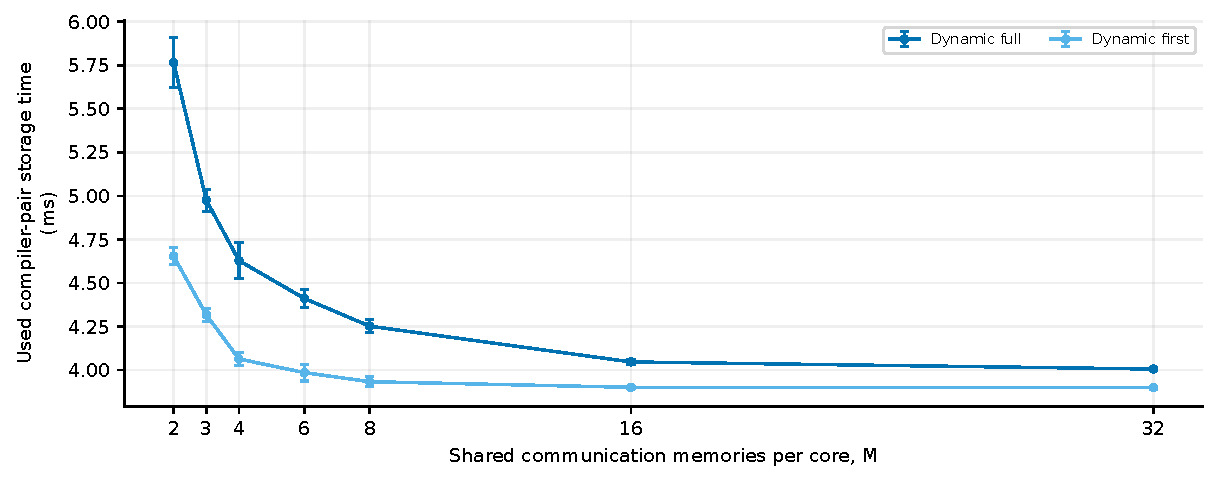
\includegraphics[width=.94\linewidth,height=.255\textheight,keepaspectratio]{figures/memory/torus_dijkstra_average_storage_time_ms.pdf}\captionof{figure}{Run-level mean and sample SD. Shared trace aliases are counted once.}\end{center}
\begin{center}{\scriptsize\setlength{\tabcolsep}{3pt}
\begin{tabular}{lrrrrr}
\toprule
M & ODG & CGP & ACGP & Dynamic full & Dynamic first \\
\midrule
2 & n/a & n/a & n/a & $5.765\pm0.143$ & $4.654\pm0.049$ \\
3 & n/a & n/a & n/a & $4.976\pm0.063$ & $4.318\pm0.038$ \\
4 & n/a & n/a & n/a & $4.629\pm0.102$ & $4.064\pm0.038$ \\
6 & n/a & n/a & n/a & $4.412\pm0.053$ & $3.986\pm0.048$ \\
8 & n/a & n/a & n/a & $4.253\pm0.038$ & $3.934\pm0.030$ \\
16 & n/a & n/a & n/a & $4.047\pm0.014$ & $3.902\pm0.007$ \\
32 & n/a & n/a & n/a & $4.006\pm0.010$ & $3.900\pm0.008$ \\
\bottomrule\end{tabular}}
\captionof{table}{Mean $\pm$ sample SD; n/a denotes a metric outside that policy's instrumentation.}
{\footnotesize\href{https://github.com/sanjeevkrishnaa/Compiler-Driven-ACE/blob/codex/ace-scheduler-correctness/docs/latex/qft96_final/data/memory_torus_dijkstra_average_storage_time_ms.csv}{Exact CSV values and sample counts}}
\end{center}
\clearpage
\subsection*{Delivered-hop throughput}
\begin{center}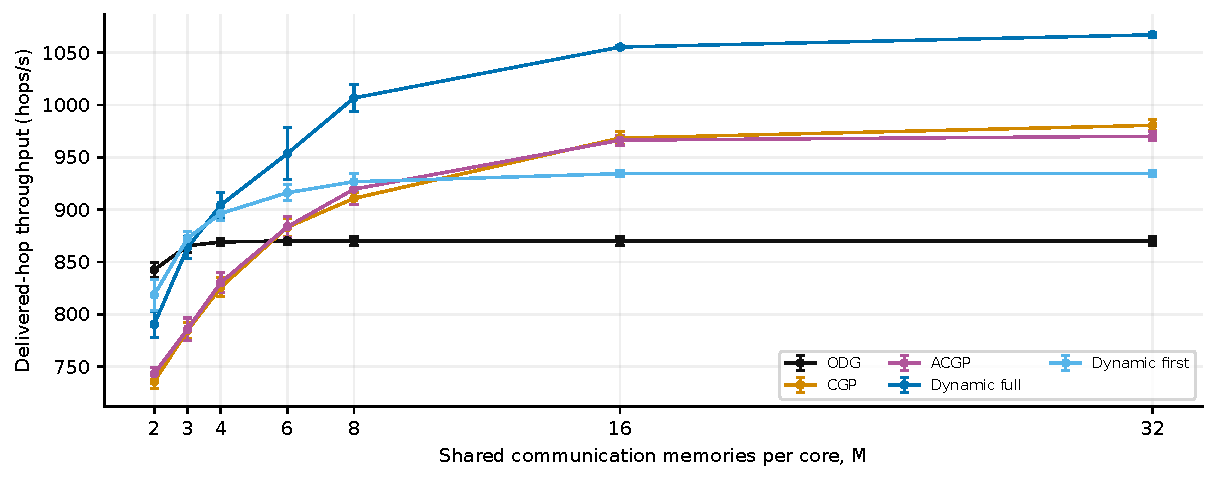
\includegraphics[width=.94\linewidth,height=.255\textheight,keepaspectratio]{figures/memory/torus_dijkstra_hop_throughput_s.pdf}\captionof{figure}{Run-level mean and sample SD. Shared trace aliases are counted once.}\end{center}
\begin{center}{\scriptsize\setlength{\tabcolsep}{3pt}
\begin{tabular}{lrrrrr}
\toprule
M & ODG & CGP & ACGP & Dynamic full & Dynamic first \\
\midrule
2 & $842.43\pm7.25$ & $735.80\pm6.96$ & $743.19\pm6.05$ & $790.29\pm12.46$ & $818.48\pm15.00$ \\
3 & $865.48\pm6.19$ & $784.59\pm7.50$ & $785.73\pm10.68$ & $863.76\pm10.61$ & $872.61\pm6.12$ \\
4 & $869.03\pm3.21$ & $825.94\pm9.10$ & $830.33\pm9.93$ & $904.41\pm11.66$ & $896.32\pm6.42$ \\
6 & $870.14\pm3.84$ & $883.17\pm8.80$ & $883.58\pm9.94$ & $953.54\pm25.00$ & $916.18\pm7.78$ \\
8 & $869.92\pm3.90$ & $910.73\pm5.76$ & $919.51\pm14.73$ & $1006.64\pm13.29$ & $926.61\pm7.45$ \\
16 & $869.92\pm3.90$ & $968.34\pm6.37$ & $966.33\pm4.87$ & $1055.31\pm1.55$ & $934.35\pm3.12$ \\
32 & $869.92\pm3.90$ & $980.54\pm5.34$ & $970.12\pm4.12$ & $1067.02\pm2.35$ & $934.50\pm3.12$ \\
\bottomrule\end{tabular}}
\captionof{table}{Mean $\pm$ sample SD; n/a denotes a metric outside that policy's instrumentation.}
{\footnotesize\href{https://github.com/sanjeevkrishnaa/Compiler-Driven-ACE/blob/codex/ace-scheduler-correctness/docs/latex/qft96_final/data/memory_torus_dijkstra_hop_throughput_s.csv}{Exact CSV values and sample counts}}
\end{center}
\subsection*{Completion fraction}
\begin{center}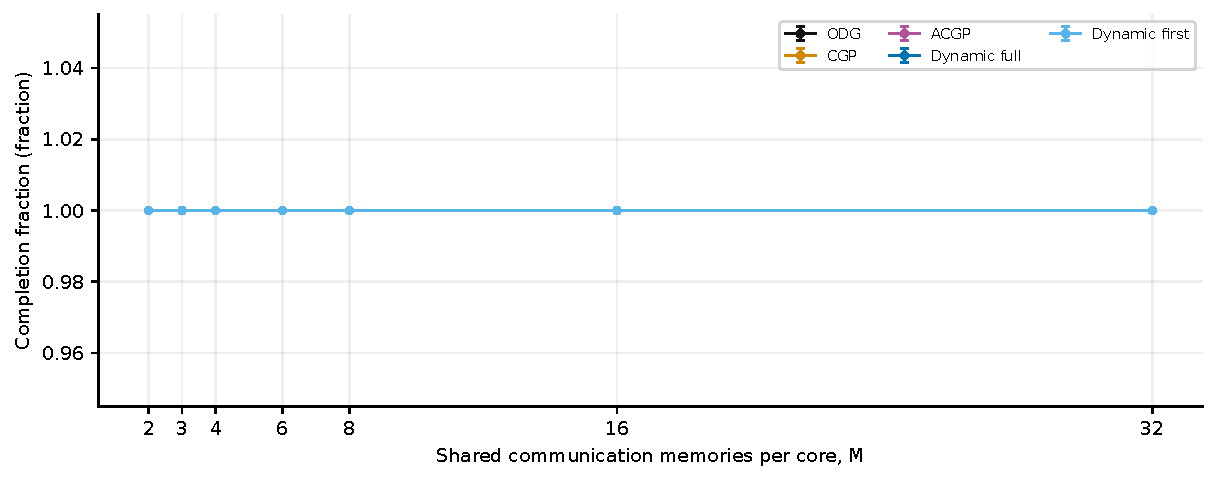
\includegraphics[width=.94\linewidth,height=.255\textheight,keepaspectratio]{figures/memory/torus_dijkstra_completion_rate.pdf}\captionof{figure}{Run-level mean and sample SD. Shared trace aliases are counted once.}\end{center}
\begin{center}{\scriptsize\setlength{\tabcolsep}{3pt}
\begin{tabular}{lrrrrr}
\toprule
M & ODG & CGP & ACGP & Dynamic full & Dynamic first \\
\midrule
2 & $1.000\pm0.000$ & $1.000\pm0.000$ & $1.000\pm0.000$ & $1.000\pm0.000$ & $1.000\pm0.000$ \\
3 & $1.000\pm0.000$ & $1.000\pm0.000$ & $1.000\pm0.000$ & $1.000\pm0.000$ & $1.000\pm0.000$ \\
4 & $1.000\pm0.000$ & $1.000\pm0.000$ & $1.000\pm0.000$ & $1.000\pm0.000$ & $1.000\pm0.000$ \\
6 & $1.000\pm0.000$ & $1.000\pm0.000$ & $1.000\pm0.000$ & $1.000\pm0.000$ & $1.000\pm0.000$ \\
8 & $1.000\pm0.000$ & $1.000\pm0.000$ & $1.000\pm0.000$ & $1.000\pm0.000$ & $1.000\pm0.000$ \\
16 & $1.000\pm0.000$ & $1.000\pm0.000$ & $1.000\pm0.000$ & $1.000\pm0.000$ & $1.000\pm0.000$ \\
32 & $1.000\pm0.000$ & $1.000\pm0.000$ & $1.000\pm0.000$ & $1.000\pm0.000$ & $1.000\pm0.000$ \\
\bottomrule\end{tabular}}
\captionof{table}{Mean $\pm$ sample SD; n/a denotes a metric outside that policy's instrumentation.}
{\footnotesize\href{https://github.com/sanjeevkrishnaa/Compiler-Driven-ACE/blob/codex/ace-scheduler-correctness/docs/latex/qft96_final/data/memory_torus_dijkstra_completion_rate.csv}{Exact CSV values and sample counts}}
\end{center}
\clearpage
\subsection*{Maximum admission wait}
\begin{center}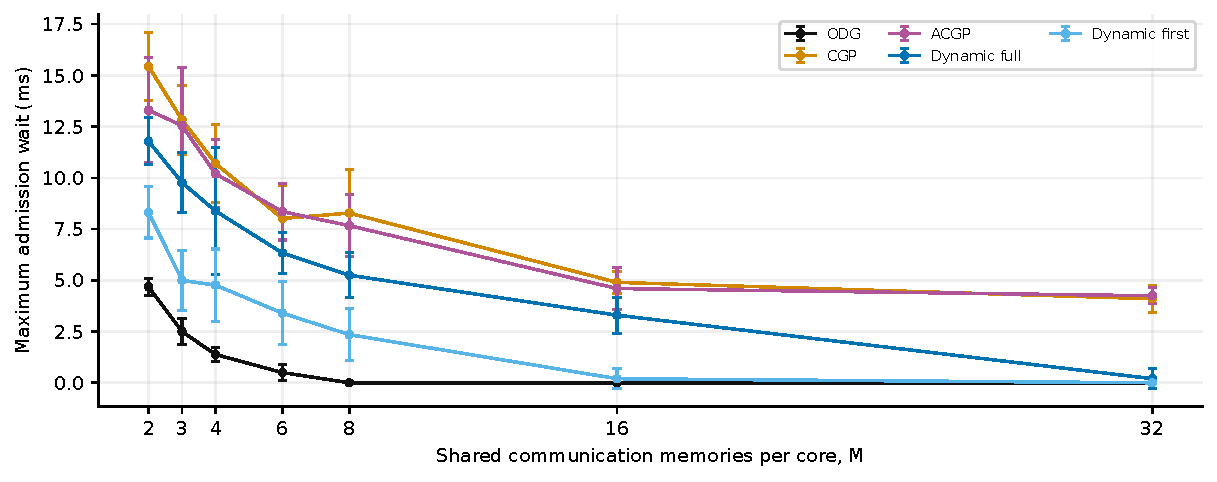
\includegraphics[width=.94\linewidth,height=.255\textheight,keepaspectratio]{figures/memory/torus_dijkstra_max_admission_wait_ms.pdf}\captionof{figure}{Run-level mean and sample SD. Shared trace aliases are counted once.}\end{center}
\begin{center}{\scriptsize\setlength{\tabcolsep}{3pt}
\begin{tabular}{lrrrrr}
\toprule
M & ODG & CGP & ACGP & Dynamic full & Dynamic first \\
\midrule
2 & $4.683\pm0.412$ & $15.434\pm1.667$ & $13.298\pm2.565$ & $11.784\pm1.150$ & $8.317\pm1.251$ \\
3 & $2.500\pm0.651$ & $12.834\pm1.680$ & $12.550\pm2.846$ & $9.767\pm1.449$ & $5.000\pm1.467$ \\
4 & $1.383\pm0.360$ & $10.700\pm1.893$ & $10.200\pm1.666$ & $8.384\pm3.097$ & $4.767\pm1.763$ \\
6 & $0.5000\pm0.4099$ & $8.017\pm1.592$ & $8.350\pm1.384$ & $6.333\pm0.983$ & $3.400\pm1.538$ \\
8 & $0.0000\pm0.0000$ & $8.284\pm2.110$ & $7.667\pm1.525$ & $5.250\pm1.106$ & $2.350\pm1.263$ \\
16 & $0.0000\pm0.0000$ & $4.900\pm0.525$ & $4.600\pm1.032$ & $3.300\pm0.874$ & $0.2000\pm0.4899$ \\
32 & $0.0000\pm0.0000$ & $4.100\pm0.651$ & $4.246\pm0.388$ & $0.2000\pm0.4899$ & $0.0000\pm0.0000$ \\
\bottomrule\end{tabular}}
\captionof{table}{Mean $\pm$ sample SD; n/a denotes a metric outside that policy's instrumentation.}
{\footnotesize\href{https://github.com/sanjeevkrishnaa/Compiler-Driven-ACE/blob/codex/ace-scheduler-correctness/docs/latex/qft96_final/data/memory_torus_dijkstra_max_admission_wait_ms.csv}{Exact CSV values and sample counts}}
\end{center}
\subsection*{Requests with admission wait}
\begin{center}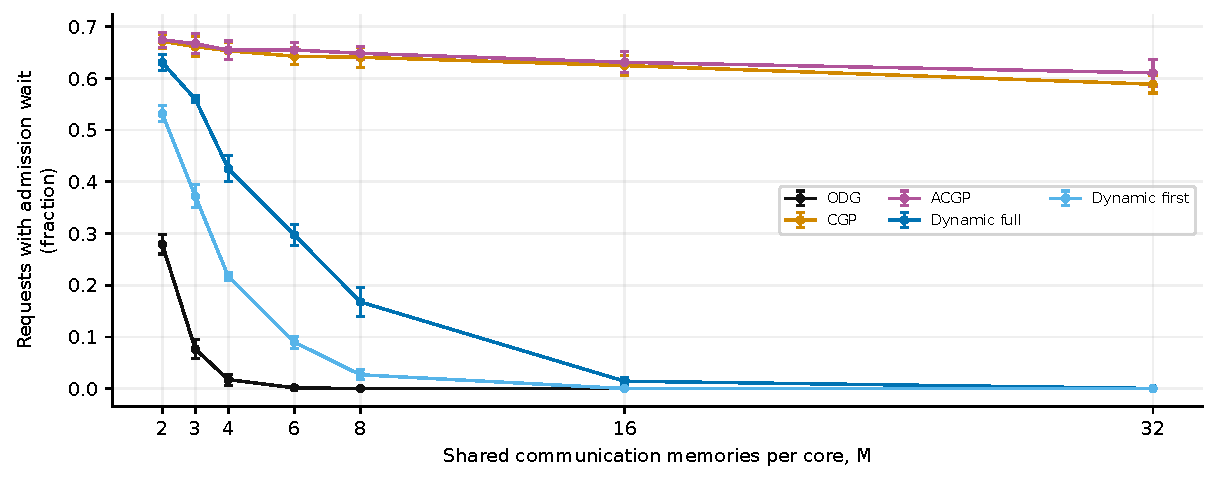
\includegraphics[width=.94\linewidth,height=.255\textheight,keepaspectratio]{figures/memory/torus_dijkstra_requests_that_waited_fraction.pdf}\captionof{figure}{Run-level mean and sample SD. Shared trace aliases are counted once.}\end{center}
\begin{center}{\scriptsize\setlength{\tabcolsep}{3pt}
\begin{tabular}{lrrrrr}
\toprule
M & ODG & CGP & ACGP & Dynamic full & Dynamic first \\
\midrule
2 & $0.2792\pm0.0188$ & $0.6719\pm0.0135$ & $0.6747\pm0.0145$ & $0.6309\pm0.0155$ & $0.5320\pm0.0149$ \\
3 & $0.0764\pm0.0188$ & $0.6615\pm0.0198$ & $0.6671\pm0.0193$ & $0.5598\pm0.0069$ & $0.3723\pm0.0222$ \\
4 & $0.0173\pm0.0107$ & $0.6536\pm0.0168$ & $0.6549\pm0.0176$ & $0.4255\pm0.0247$ & $0.2168\pm0.0068$ \\
6 & $0.0015\pm0.0015$ & $0.6430\pm0.0164$ & $0.6552\pm0.0148$ & $0.2974\pm0.0204$ & $0.0898\pm0.0116$ \\
8 & $0.0000\pm0.0000$ & $0.6409\pm0.0193$ & $0.6486\pm0.0127$ & $0.1677\pm0.0277$ & $0.0267\pm0.0095$ \\
16 & $0.0000\pm0.0000$ & $0.6250\pm0.0193$ & $0.6313\pm0.0202$ & $0.0143\pm0.0070$ & $0.0001\pm0.0003$ \\
32 & $0.0000\pm0.0000$ & $0.5888\pm0.0169$ & $0.6108\pm0.0253$ & $0.0002\pm0.0005$ & $0.0000\pm0.0000$ \\
\bottomrule\end{tabular}}
\captionof{table}{Mean $\pm$ sample SD; n/a denotes a metric outside that policy's instrumentation.}
{\footnotesize\href{https://github.com/sanjeevkrishnaa/Compiler-Driven-ACE/blob/codex/ace-scheduler-correctness/docs/latex/qft96_final/data/memory_torus_dijkstra_requests_that_waited_fraction.csv}{Exact CSV values and sample counts}}
\end{center}
\clearpage
\subsection*{Recorded reservation-setup counter}
\begin{center}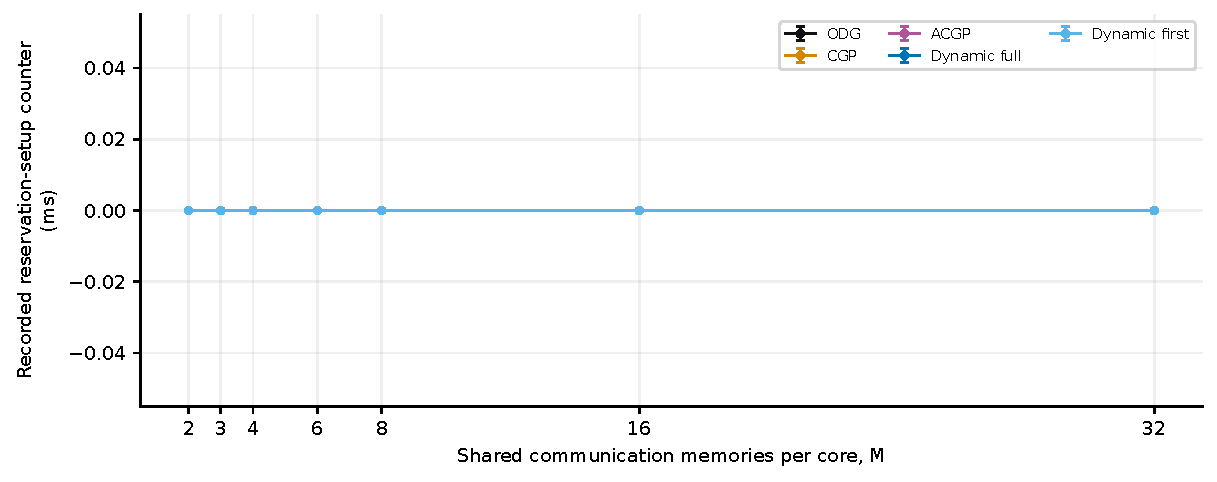
\includegraphics[width=.94\linewidth,height=.255\textheight,keepaspectratio]{figures/memory/torus_dijkstra_avg_reservation_setup_time_ms.pdf}\captionof{figure}{Run-level mean and sample SD. Shared trace aliases are counted once.}\end{center}
\begin{center}{\scriptsize\setlength{\tabcolsep}{3pt}
\begin{tabular}{lrrrrr}
\toprule
M & ODG & CGP & ACGP & Dynamic full & Dynamic first \\
\midrule
2 & $0.0000\pm0.0000$ & $0.0000\pm0.0000$ & $0.0000\pm0.0000$ & $0.0000\pm0.0000$ & $0.0000\pm0.0000$ \\
3 & $0.0000\pm0.0000$ & $0.0000\pm0.0000$ & $0.0000\pm0.0000$ & $0.0000\pm0.0000$ & $0.0000\pm0.0000$ \\
4 & $0.0000\pm0.0000$ & $0.0000\pm0.0000$ & $0.0000\pm0.0000$ & $0.0000\pm0.0000$ & $0.0000\pm0.0000$ \\
6 & $0.0000\pm0.0000$ & $0.0000\pm0.0000$ & $0.0000\pm0.0000$ & $0.0000\pm0.0000$ & $0.0000\pm0.0000$ \\
8 & $0.0000\pm0.0000$ & $0.0000\pm0.0000$ & $0.0000\pm0.0000$ & $0.0000\pm0.0000$ & $0.0000\pm0.0000$ \\
16 & $0.0000\pm0.0000$ & $0.0000\pm0.0000$ & $0.0000\pm0.0000$ & $0.0000\pm0.0000$ & $0.0000\pm0.0000$ \\
32 & $0.0000\pm0.0000$ & $0.0000\pm0.0000$ & $0.0000\pm0.0000$ & $0.0000\pm0.0000$ & $0.0000\pm0.0000$ \\
\bottomrule\end{tabular}}
\captionof{table}{Mean $\pm$ sample SD; n/a denotes a metric outside that policy's instrumentation.}
{\footnotesize\href{https://github.com/sanjeevkrishnaa/Compiler-Driven-ACE/blob/codex/ace-scheduler-correctness/docs/latex/qft96_final/data/memory_torus_dijkstra_avg_reservation_setup_time_ms.csv}{Exact CSV values and sample counts}}
\end{center}
\subsection*{Mean generation/service time}
\begin{center}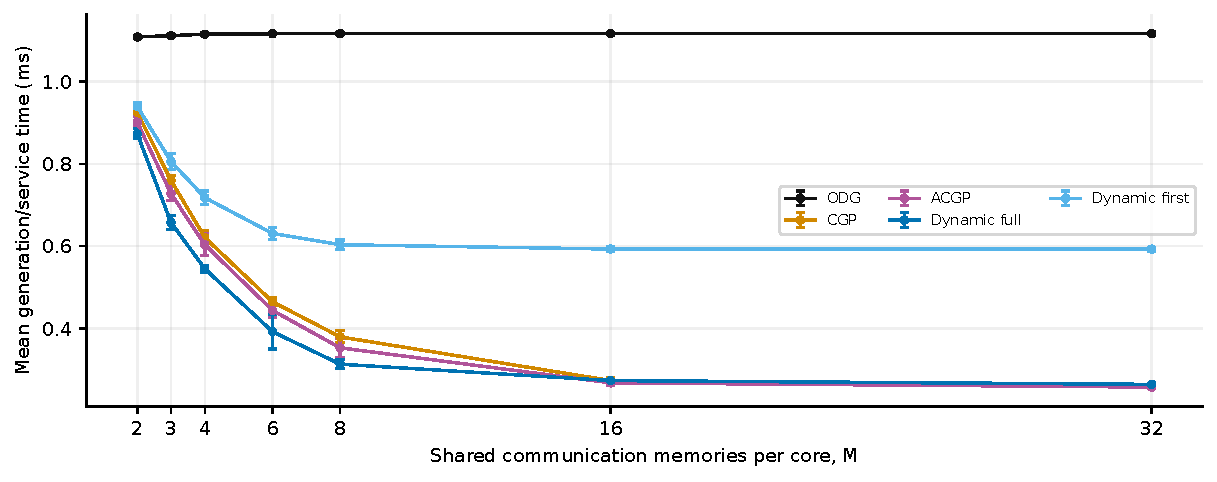
\includegraphics[width=.94\linewidth,height=.255\textheight,keepaspectratio]{figures/memory/torus_dijkstra_avg_entanglement_generation_time_ms.pdf}\captionof{figure}{Run-level mean and sample SD. Shared trace aliases are counted once.}\end{center}
\begin{center}{\scriptsize\setlength{\tabcolsep}{3pt}
\begin{tabular}{lrrrrr}
\toprule
M & ODG & CGP & ACGP & Dynamic full & Dynamic first \\
\midrule
2 & $1.109\pm0.002$ & $0.9258\pm0.0098$ & $0.9008\pm0.0134$ & $0.8732\pm0.0120$ & $0.9398\pm0.0083$ \\
3 & $1.112\pm0.002$ & $0.7595\pm0.0113$ & $0.7274\pm0.0175$ & $0.6575\pm0.0170$ & $0.8057\pm0.0195$ \\
4 & $1.115\pm0.003$ & $0.6209\pm0.0178$ & $0.6037\pm0.0270$ & $0.5449\pm0.0083$ & $0.7179\pm0.0161$ \\
6 & $1.116\pm0.003$ & $0.4647\pm0.0095$ & $0.4438\pm0.0180$ & $0.3920\pm0.0422$ & $0.6309\pm0.0137$ \\
8 & $1.117\pm0.003$ & $0.3794\pm0.0145$ & $0.3528\pm0.0236$ & $0.3130\pm0.0110$ & $0.6035\pm0.0115$ \\
16 & $1.117\pm0.003$ & $0.2731\pm0.0078$ & $0.2676\pm0.0056$ & $0.2731\pm0.0017$ & $0.5929\pm0.0051$ \\
32 & $1.117\pm0.003$ & $0.2609\pm0.0041$ & $0.2573\pm0.0040$ & $0.2639\pm0.0020$ & $0.5928\pm0.0050$ \\
\bottomrule\end{tabular}}
\captionof{table}{Mean $\pm$ sample SD; n/a denotes a metric outside that policy's instrumentation.}
{\footnotesize\href{https://github.com/sanjeevkrishnaa/Compiler-Driven-ACE/blob/codex/ace-scheduler-correctness/docs/latex/qft96_final/data/memory_torus_dijkstra_avg_entanglement_generation_time_ms.csv}{Exact CSV values and sample counts}}
\end{center}
\clearpage
\subsection*{Recorded retry-wait time}
\begin{center}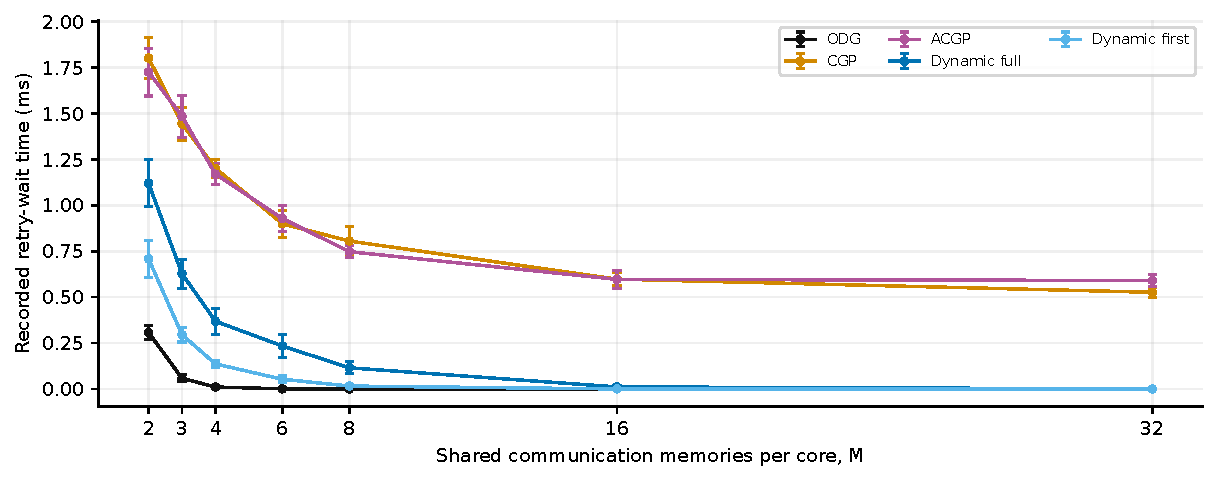
\includegraphics[width=.94\linewidth,height=.255\textheight,keepaspectratio]{figures/memory/torus_dijkstra_avg_retry_wait_time_ms.pdf}\captionof{figure}{Run-level mean and sample SD. Shared trace aliases are counted once.}\end{center}
\begin{center}{\scriptsize\setlength{\tabcolsep}{3pt}
\begin{tabular}{lrrrrr}
\toprule
M & ODG & CGP & ACGP & Dynamic full & Dynamic first \\
\midrule
2 & $0.3075\pm0.0402$ & $1.801\pm0.111$ & $1.725\pm0.131$ & $1.120\pm0.128$ & $0.7084\pm0.1012$ \\
3 & $0.0581\pm0.0199$ & $1.443\pm0.088$ & $1.484\pm0.115$ & $0.6269\pm0.0805$ & $0.2953\pm0.0394$ \\
4 & $0.0106\pm0.0073$ & $1.201\pm0.049$ & $1.170\pm0.057$ & $0.3686\pm0.0716$ & $0.1364\pm0.0186$ \\
6 & $0.0006\pm0.0007$ & $0.8995\pm0.0741$ & $0.9284\pm0.0687$ & $0.2339\pm0.0607$ & $0.0528\pm0.0182$ \\
8 & $0.0000\pm0.0000$ & $0.8054\pm0.0791$ & $0.7476\pm0.0324$ & $0.1153\pm0.0323$ & $0.0159\pm0.0079$ \\
16 & $0.0000\pm0.0000$ & $0.5980\pm0.0365$ & $0.5966\pm0.0471$ & $0.0113\pm0.0051$ & $0.0001\pm0.0002$ \\
32 & $0.0000\pm0.0000$ & $0.5263\pm0.0277$ & $0.5905\pm0.0329$ & $0.0001\pm0.0004$ & $0.0000\pm0.0000$ \\
\bottomrule\end{tabular}}
\captionof{table}{Mean $\pm$ sample SD; n/a denotes a metric outside that policy's instrumentation.}
{\footnotesize\href{https://github.com/sanjeevkrishnaa/Compiler-Driven-ACE/blob/codex/ace-scheduler-correctness/docs/latex/qft96_final/data/memory_torus_dijkstra_avg_retry_wait_time_ms.csv}{Exact CSV values and sample counts}}
\end{center}
\subsection*{Request retries}
\begin{center}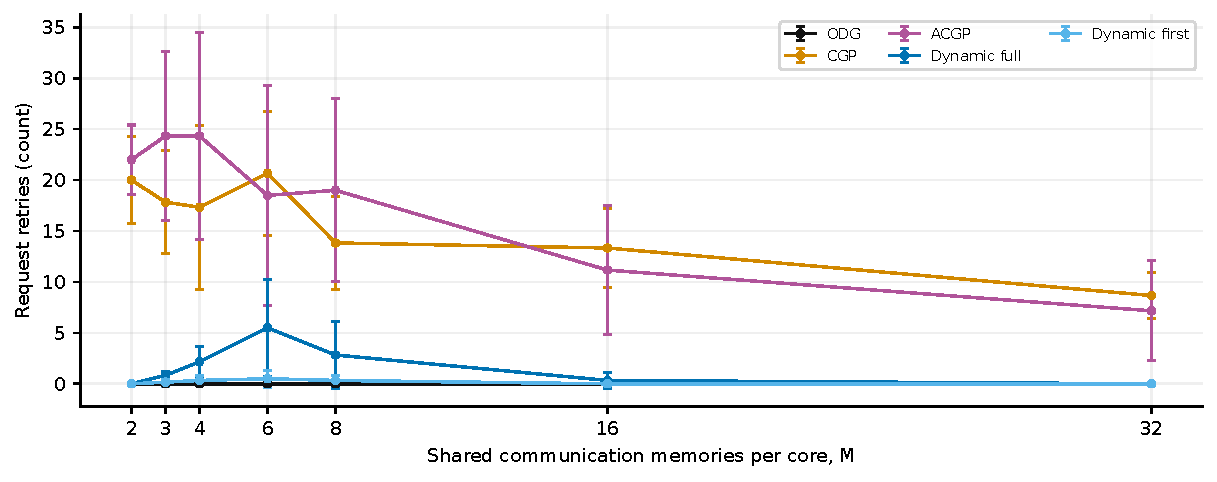
\includegraphics[width=.94\linewidth,height=.255\textheight,keepaspectratio]{figures/memory/torus_dijkstra_total_retries.pdf}\captionof{figure}{Run-level mean and sample SD. Shared trace aliases are counted once.}\end{center}
\begin{center}{\scriptsize\setlength{\tabcolsep}{3pt}
\begin{tabular}{lrrrrr}
\toprule
M & ODG & CGP & ACGP & Dynamic full & Dynamic first \\
\midrule
2 & $0.0000\pm0.0000$ & $20.000\pm4.243$ & $22.000\pm3.406$ & $0.0000\pm0.0000$ & $0.0000\pm0.0000$ \\
3 & $0.0000\pm0.0000$ & $17.833\pm5.037$ & $24.333\pm8.311$ & $0.8333\pm0.4082$ & $0.1667\pm0.4082$ \\
4 & $0.0000\pm0.0000$ & $17.333\pm8.042$ & $24.333\pm10.172$ & $2.167\pm1.472$ & $0.3333\pm0.5164$ \\
6 & $0.0000\pm0.0000$ & $20.667\pm6.088$ & $18.500\pm10.784$ & $5.500\pm4.764$ & $0.5000\pm0.8367$ \\
8 & $0.0000\pm0.0000$ & $13.833\pm4.535$ & $19.000\pm8.989$ & $2.833\pm3.312$ & $0.3333\pm0.5164$ \\
16 & $0.0000\pm0.0000$ & $13.333\pm3.882$ & $11.167\pm6.369$ & $0.3333\pm0.8165$ & $0.0000\pm0.0000$ \\
32 & $0.0000\pm0.0000$ & $8.667\pm2.251$ & $7.167\pm4.916$ & $0.0000\pm0.0000$ & $0.0000\pm0.0000$ \\
\bottomrule\end{tabular}}
\captionof{table}{Mean $\pm$ sample SD; n/a denotes a metric outside that policy's instrumentation.}
{\footnotesize\href{https://github.com/sanjeevkrishnaa/Compiler-Driven-ACE/blob/codex/ace-scheduler-correctness/docs/latex/qft96_final/data/memory_torus_dijkstra_total_retries.csv}{Exact CSV values and sample counts}}
\end{center}
\clearpage
\subsection*{Requests with retries}
\begin{center}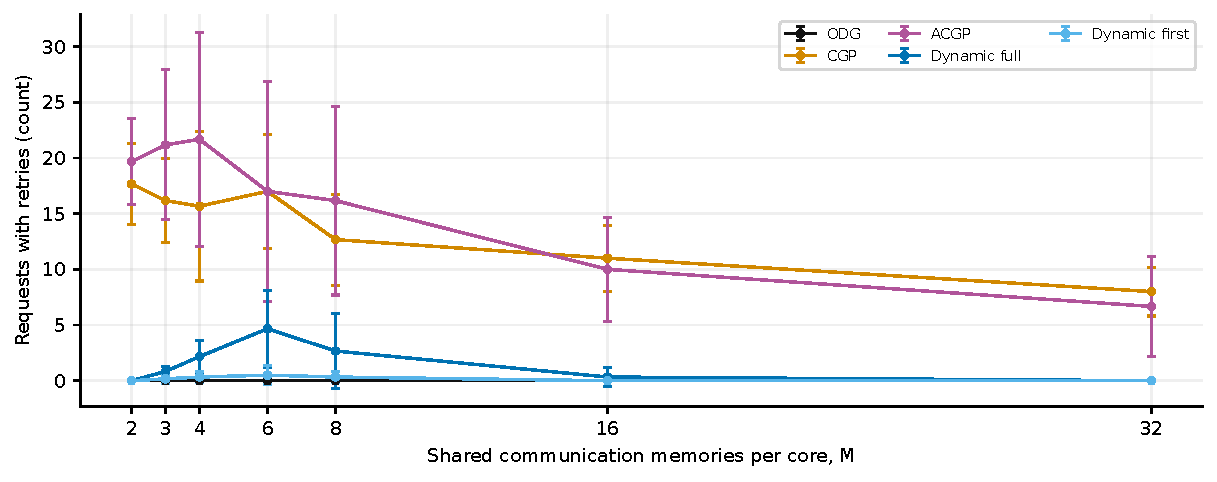
\includegraphics[width=.94\linewidth,height=.255\textheight,keepaspectratio]{figures/memory/torus_dijkstra_requests_with_retries.pdf}\captionof{figure}{Run-level mean and sample SD. Shared trace aliases are counted once.}\end{center}
\begin{center}{\scriptsize\setlength{\tabcolsep}{3pt}
\begin{tabular}{lrrrrr}
\toprule
M & ODG & CGP & ACGP & Dynamic full & Dynamic first \\
\midrule
2 & $0.0000\pm0.0000$ & $17.667\pm3.615$ & $19.667\pm3.882$ & $0.0000\pm0.0000$ & $0.0000\pm0.0000$ \\
3 & $0.0000\pm0.0000$ & $16.167\pm3.764$ & $21.167\pm6.735$ & $0.8333\pm0.4082$ & $0.1667\pm0.4082$ \\
4 & $0.0000\pm0.0000$ & $15.667\pm6.713$ & $21.667\pm9.606$ & $2.167\pm1.472$ & $0.3333\pm0.5164$ \\
6 & $0.0000\pm0.0000$ & $17.000\pm5.138$ & $17.000\pm9.859$ & $4.667\pm3.445$ & $0.5000\pm0.8367$ \\
8 & $0.0000\pm0.0000$ & $12.667\pm4.082$ & $16.167\pm8.472$ & $2.667\pm3.386$ & $0.3333\pm0.5164$ \\
16 & $0.0000\pm0.0000$ & $11.000\pm2.966$ & $10.000\pm4.690$ & $0.3333\pm0.8165$ & $0.0000\pm0.0000$ \\
32 & $0.0000\pm0.0000$ & $8.000\pm2.191$ & $6.667\pm4.457$ & $0.0000\pm0.0000$ & $0.0000\pm0.0000$ \\
\bottomrule\end{tabular}}
\captionof{table}{Mean $\pm$ sample SD; n/a denotes a metric outside that policy's instrumentation.}
{\footnotesize\href{https://github.com/sanjeevkrishnaa/Compiler-Driven-ACE/blob/codex/ace-scheduler-correctness/docs/latex/qft96_final/data/memory_torus_dijkstra_requests_with_retries.csv}{Exact CSV values and sample counts}}
\end{center}
\subsection*{Native-protocol generated-pair counter}
\begin{center}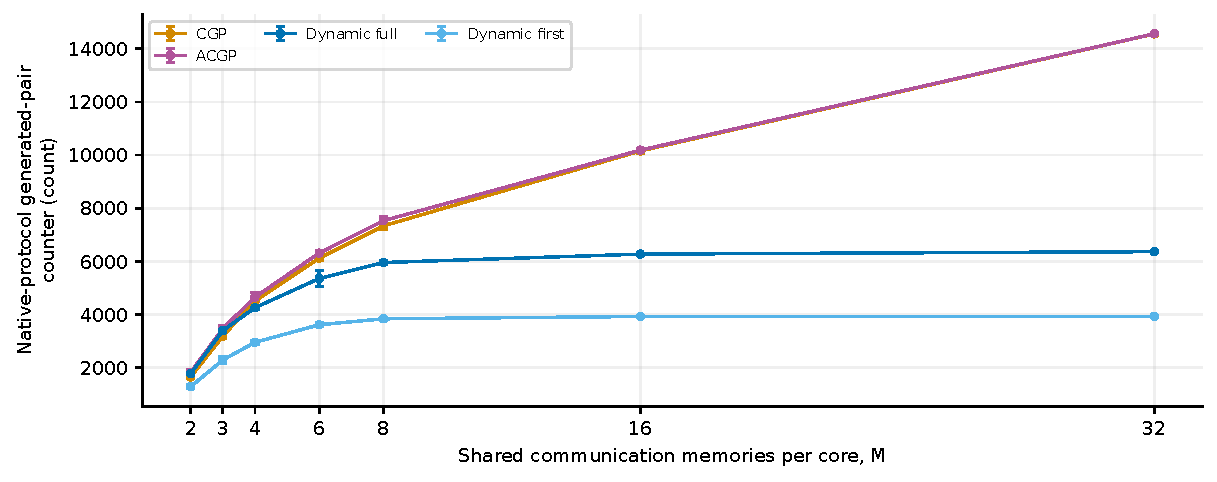
\includegraphics[width=.94\linewidth,height=.255\textheight,keepaspectratio]{figures/memory/torus_dijkstra_protocol_generated_pairs.pdf}\captionof{figure}{Run-level mean and sample SD. Shared trace aliases are counted once.}\end{center}
\begin{center}{\scriptsize\setlength{\tabcolsep}{3pt}
\begin{tabular}{lrrrrr}
\toprule
M & ODG & CGP & ACGP & Dynamic full & Dynamic first \\
\midrule
2 & n/a & $1652.00\pm60.97$ & $1829.67\pm107.13$ & $1779.67\pm89.20$ & $1288.00\pm78.61$ \\
3 & n/a & $3188.00\pm75.06$ & $3470.67\pm132.90$ & $3397.67\pm113.75$ & $2291.67\pm114.52$ \\
4 & n/a & $4501.33\pm157.77$ & $4652.00\pm162.69$ & $4258.00\pm66.86$ & $2954.33\pm76.20$ \\
6 & n/a & $6123.67\pm88.89$ & $6312.67\pm99.87$ & $5356.00\pm294.69$ & $3616.00\pm74.66$ \\
8 & n/a & $7334.00\pm115.54$ & $7529.67\pm156.25$ & $5956.33\pm73.28$ & $3840.00\pm57.09$ \\
16 & n/a & $10153.00\pm91.28$ & $10183.33\pm43.50$ & $6273.33\pm22.97$ & $3927.33\pm6.53$ \\
32 & n/a & $14558.00\pm57.06$ & $14560.00\pm36.60$ & $6366.00\pm10.58$ & $3930.00\pm0.00$ \\
\bottomrule\end{tabular}}
\captionof{table}{Mean $\pm$ sample SD; n/a denotes a metric outside that policy's instrumentation.}
{\footnotesize\href{https://github.com/sanjeevkrishnaa/Compiler-Driven-ACE/blob/codex/ace-scheduler-correctness/docs/latex/qft96_final/data/memory_torus_dijkstra_protocol_generated_pairs.csv}{Exact CSV values and sample counts}}
\end{center}
\clearpage
\subsection*{Native-protocol used-pair counter}
\begin{center}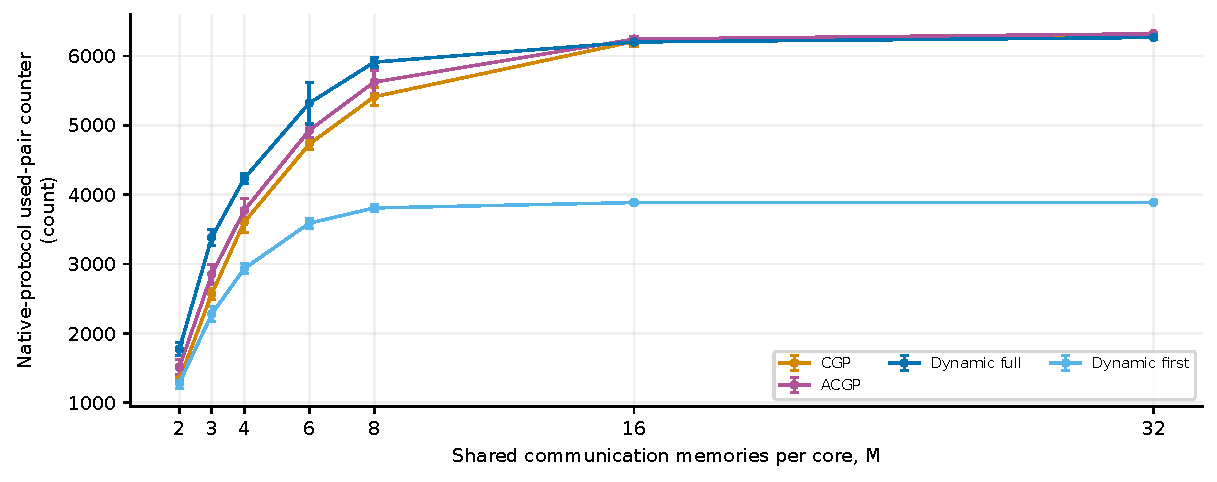
\includegraphics[width=.94\linewidth,height=.255\textheight,keepaspectratio]{figures/memory/torus_dijkstra_protocol_used_pairs.pdf}\captionof{figure}{Run-level mean and sample SD. Shared trace aliases are counted once.}\end{center}
\begin{center}{\scriptsize\setlength{\tabcolsep}{3pt}
\begin{tabular}{lrrrrr}
\toprule
M & ODG & CGP & ACGP & Dynamic full & Dynamic first \\
\midrule
2 & n/a & $1331.33\pm61.20$ & $1513.00\pm106.33$ & $1773.00\pm91.14$ & $1282.00\pm79.96$ \\
3 & n/a & $2572.33\pm80.27$ & $2852.67\pm140.61$ & $3385.33\pm114.81$ & $2279.67\pm114.47$ \\
4 & n/a & $3605.00\pm153.37$ & $3772.00\pm173.13$ & $4235.00\pm72.58$ & $2934.67\pm74.44$ \\
6 & n/a & $4728.33\pm81.39$ & $4928.00\pm99.67$ & $5320.00\pm300.26$ & $3589.00\pm72.19$ \\
8 & n/a & $5412.67\pm130.97$ & $5624.33\pm164.39$ & $5911.33\pm70.13$ & $3808.67\pm55.48$ \\
16 & n/a & $6209.33\pm69.28$ & $6243.00\pm39.61$ & $6201.67\pm24.05$ & $3886.67\pm7.87$ \\
32 & n/a & $6291.00\pm23.07$ & $6321.33\pm19.95$ & $6267.00\pm16.82$ & $3889.33\pm4.84$ \\
\bottomrule\end{tabular}}
\captionof{table}{Mean $\pm$ sample SD; n/a denotes a metric outside that policy's instrumentation.}
{\footnotesize\href{https://github.com/sanjeevkrishnaa/Compiler-Driven-ACE/blob/codex/ace-scheduler-correctness/docs/latex/qft96_final/data/memory_torus_dijkstra_protocol_used_pairs.csv}{Exact CSV values and sample counts}}
\end{center}
\subsection*{Native-protocol unused-pair counter}
\begin{center}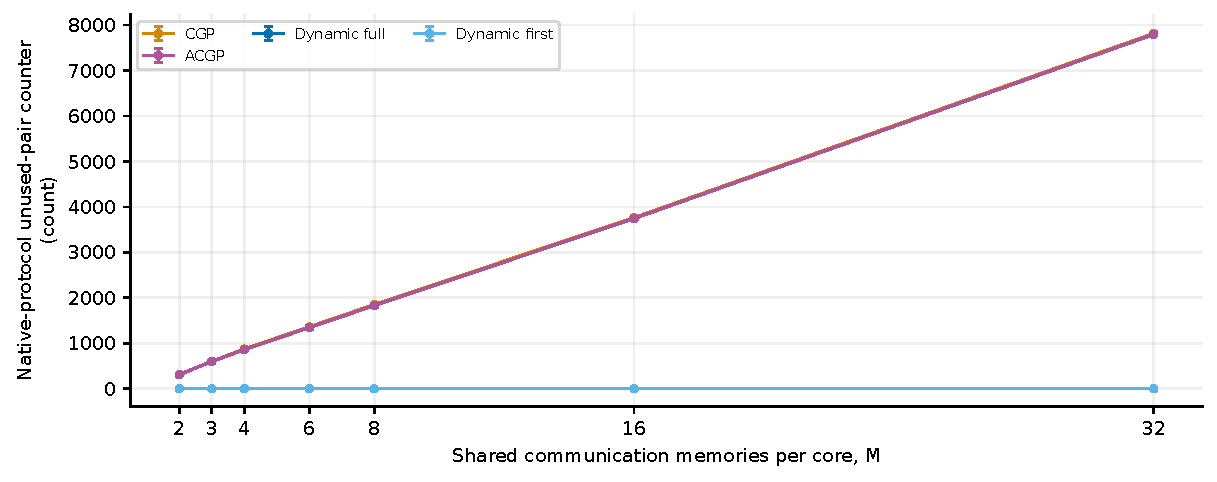
\includegraphics[width=.94\linewidth,height=.255\textheight,keepaspectratio]{figures/memory/torus_dijkstra_protocol_unused_pairs.pdf}\captionof{figure}{Run-level mean and sample SD. Shared trace aliases are counted once.}\end{center}
\begin{center}{\scriptsize\setlength{\tabcolsep}{3pt}
\begin{tabular}{lrrrrr}
\toprule
M & ODG & CGP & ACGP & Dynamic full & Dynamic first \\
\midrule
2 & n/a & $313.00\pm4.69$ & $311.33\pm3.01$ & $0.0000\pm0.0000$ & $0.0000\pm0.0000$ \\
3 & n/a & $600.00\pm13.62$ & $601.67\pm14.11$ & $0.0000\pm0.0000$ & $0.0000\pm0.0000$ \\
4 & n/a & $871.67\pm5.85$ & $861.67\pm21.22$ & $0.0000\pm0.0000$ & $0.0000\pm0.0000$ \\
6 & n/a & $1358.33\pm39.10$ & $1347.00\pm43.43$ & $0.0000\pm0.0000$ & $0.0000\pm0.0000$ \\
8 & n/a & $1847.67\pm9.42$ & $1830.67\pm46.66$ & $0.0000\pm0.0000$ & $0.0000\pm0.0000$ \\
16 & n/a & $3759.67\pm12.16$ & $3744.67\pm14.07$ & $0.0000\pm0.0000$ & $0.0000\pm0.0000$ \\
32 & n/a & $7811.33\pm26.97$ & $7793.67\pm11.48$ & $0.0000\pm0.0000$ & $0.0000\pm0.0000$ \\
\bottomrule\end{tabular}}
\captionof{table}{Mean $\pm$ sample SD; n/a denotes a metric outside that policy's instrumentation.}
{\footnotesize\href{https://github.com/sanjeevkrishnaa/Compiler-Driven-ACE/blob/codex/ace-scheduler-correctness/docs/latex/qft96_final/data/memory_torus_dijkstra_protocol_unused_pairs.csv}{Exact CSV values and sample counts}}
\end{center}
\clearpage
\subsection*{Scheduled compiler preparations}
\begin{center}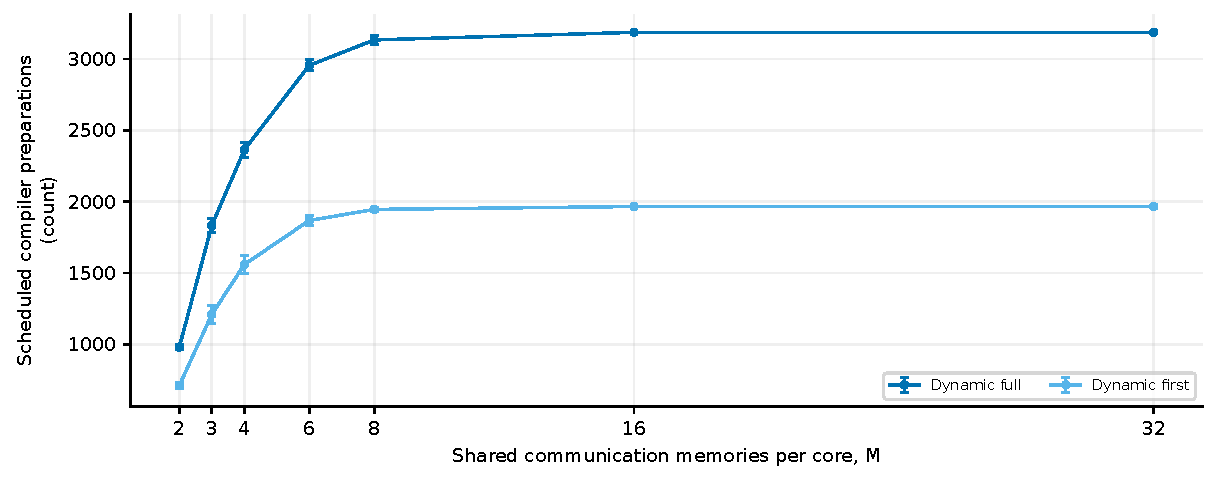
\includegraphics[width=.94\linewidth,height=.255\textheight,keepaspectratio]{figures/memory/torus_dijkstra_scheduled_preparations.pdf}\captionof{figure}{Run-level mean and sample SD. Shared trace aliases are counted once.}\end{center}
\begin{center}{\scriptsize\setlength{\tabcolsep}{3pt}
\begin{tabular}{lrrrrr}
\toprule
M & ODG & CGP & ACGP & Dynamic full & Dynamic first \\
\midrule
2 & n/a & n/a & n/a & $979.67\pm16.26$ & $710.33\pm22.74$ \\
3 & n/a & n/a & n/a & $1831.33\pm49.77$ & $1208.67\pm61.19$ \\
4 & n/a & n/a & n/a & $2362.00\pm53.04$ & $1558.00\pm60.90$ \\
6 & n/a & n/a & n/a & $2954.33\pm38.91$ & $1867.00\pm37.19$ \\
8 & n/a & n/a & n/a & $3132.67\pm32.62$ & $1944.67\pm13.89$ \\
16 & n/a & n/a & n/a & $3186.00\pm0.00$ & $1965.00\pm0.00$ \\
32 & n/a & n/a & n/a & $3186.00\pm0.00$ & $1965.00\pm0.00$ \\
\bottomrule\end{tabular}}
\captionof{table}{Mean $\pm$ sample SD; n/a denotes a metric outside that policy's instrumentation.}
{\footnotesize\href{https://github.com/sanjeevkrishnaa/Compiler-Driven-ACE/blob/codex/ace-scheduler-correctness/docs/latex/qft96_final/data/memory_torus_dijkstra_scheduled_preparations.csv}{Exact CSV values and sample counts}}
\end{center}
\subsection*{Planner-blocked preparations}
\begin{center}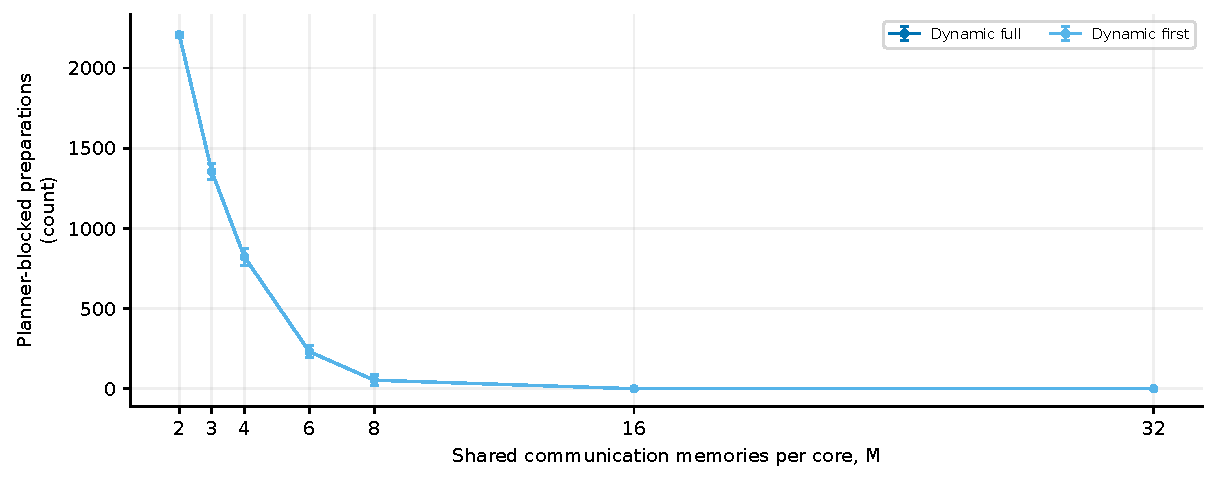
\includegraphics[width=.94\linewidth,height=.255\textheight,keepaspectratio]{figures/memory/torus_dijkstra_planner_blocked_preparations.pdf}\captionof{figure}{Run-level mean and sample SD. Shared trace aliases are counted once.}\end{center}
\begin{center}{\scriptsize\setlength{\tabcolsep}{3pt}
\begin{tabular}{lrrrrr}
\toprule
M & ODG & CGP & ACGP & Dynamic full & Dynamic first \\
\midrule
2 & n/a & n/a & n/a & $2206.33\pm16.26$ & $2206.33\pm16.26$ \\
3 & n/a & n/a & n/a & $1354.67\pm49.77$ & $1354.67\pm49.77$ \\
4 & n/a & n/a & n/a & $824.00\pm53.04$ & $824.00\pm53.04$ \\
6 & n/a & n/a & n/a & $231.67\pm38.91$ & $231.67\pm38.91$ \\
8 & n/a & n/a & n/a & $53.333\pm32.623$ & $53.333\pm32.623$ \\
16 & n/a & n/a & n/a & $0.0000\pm0.0000$ & $0.0000\pm0.0000$ \\
32 & n/a & n/a & n/a & $0.0000\pm0.0000$ & $0.0000\pm0.0000$ \\
\bottomrule\end{tabular}}
\captionof{table}{Mean $\pm$ sample SD; n/a denotes a metric outside that policy's instrumentation.}
{\footnotesize\href{https://github.com/sanjeevkrishnaa/Compiler-Driven-ACE/blob/codex/ace-scheduler-correctness/docs/latex/qft96_final/data/memory_torus_dijkstra_planner_blocked_preparations.csv}{Exact CSV values and sample counts}}
\end{center}
\clearpage
\subsection*{Planner peak compiler memory}
\begin{center}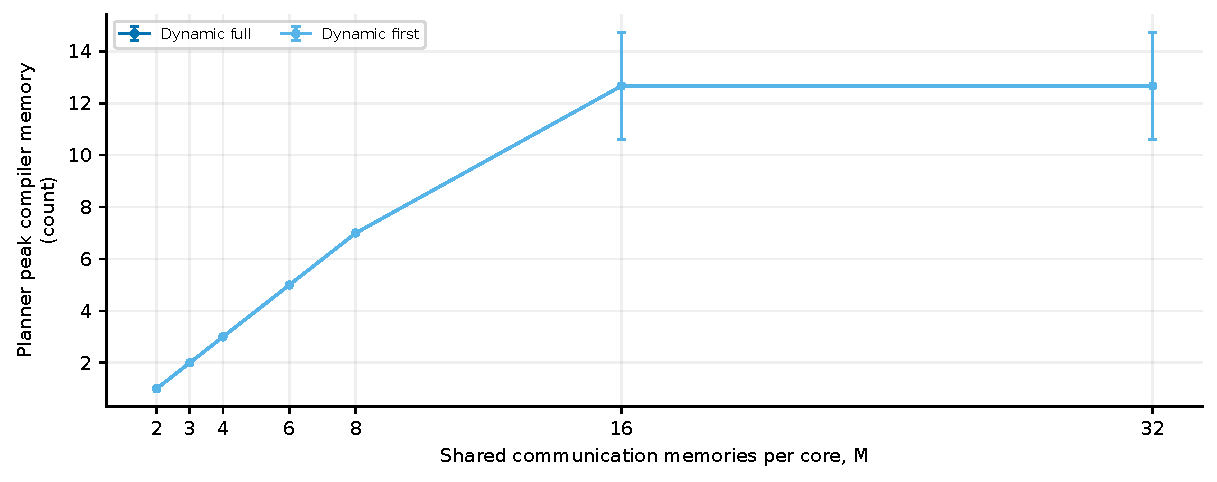
\includegraphics[width=.94\linewidth,height=.255\textheight,keepaspectratio]{figures/memory/torus_dijkstra_planner_peak_compiler_memory_per_core.pdf}\captionof{figure}{Run-level mean and sample SD. Shared trace aliases are counted once.}\end{center}
\begin{center}{\scriptsize\setlength{\tabcolsep}{3pt}
\begin{tabular}{lrrrrr}
\toprule
M & ODG & CGP & ACGP & Dynamic full & Dynamic first \\
\midrule
2 & n/a & n/a & n/a & $1.000\pm0.000$ & $1.000\pm0.000$ \\
3 & n/a & n/a & n/a & $2.000\pm0.000$ & $2.000\pm0.000$ \\
4 & n/a & n/a & n/a & $3.000\pm0.000$ & $3.000\pm0.000$ \\
6 & n/a & n/a & n/a & $5.000\pm0.000$ & $5.000\pm0.000$ \\
8 & n/a & n/a & n/a & $7.000\pm0.000$ & $7.000\pm0.000$ \\
16 & n/a & n/a & n/a & $12.667\pm2.066$ & $12.667\pm2.066$ \\
32 & n/a & n/a & n/a & $12.667\pm2.066$ & $12.667\pm2.066$ \\
\bottomrule\end{tabular}}
\captionof{table}{Mean $\pm$ sample SD; n/a denotes a metric outside that policy's instrumentation.}
{\footnotesize\href{https://github.com/sanjeevkrishnaa/Compiler-Driven-ACE/blob/codex/ace-scheduler-correctness/docs/latex/qft96_final/data/memory_torus_dijkstra_planner_peak_compiler_memory_per_core.csv}{Exact CSV values and sample counts}}
\end{center}
\subsection*{Compiler preparation admission attempts}
\begin{center}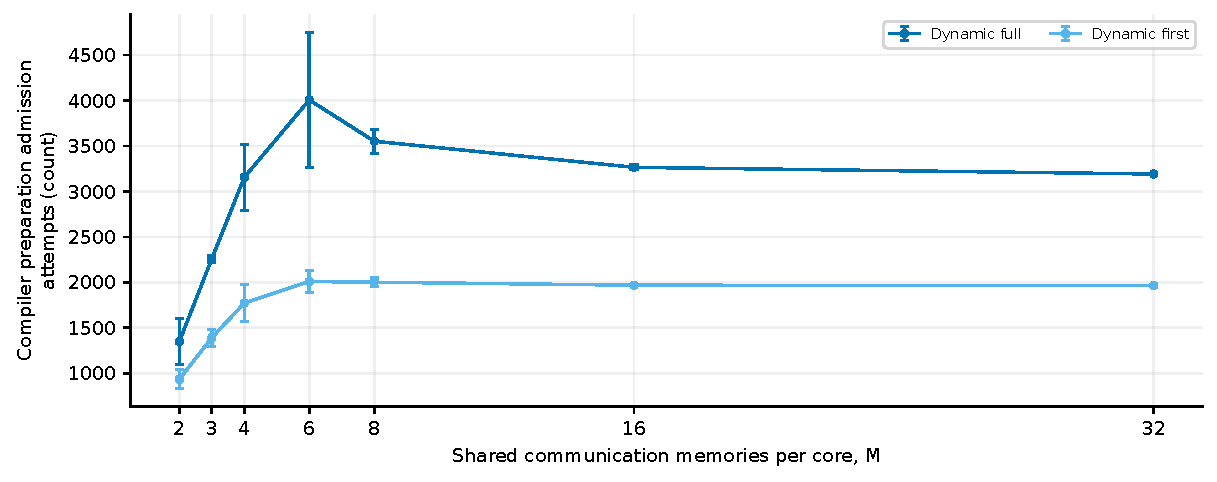
\includegraphics[width=.94\linewidth,height=.255\textheight,keepaspectratio]{figures/memory/torus_dijkstra_runtime_admission_attempts.pdf}\captionof{figure}{Run-level mean and sample SD. Shared trace aliases are counted once.}\end{center}
\begin{center}{\scriptsize\setlength{\tabcolsep}{3pt}
\begin{tabular}{lrrrrr}
\toprule
M & ODG & CGP & ACGP & Dynamic full & Dynamic first \\
\midrule
2 & n/a & n/a & n/a & $1348.50\pm256.88$ & $933.83\pm104.36$ \\
3 & n/a & n/a & n/a & $2258.33\pm40.18$ & $1390.67\pm91.59$ \\
4 & n/a & n/a & n/a & $3154.33\pm366.09$ & $1771.00\pm205.41$ \\
6 & n/a & n/a & n/a & $4005.67\pm743.63$ & $2008.83\pm119.46$ \\
8 & n/a & n/a & n/a & $3552.00\pm131.03$ & $2001.33\pm46.02$ \\
16 & n/a & n/a & n/a & $3264.50\pm28.47$ & $1968.33\pm8.16$ \\
32 & n/a & n/a & n/a & $3190.83\pm10.01$ & $1965.00\pm0.00$ \\
\bottomrule\end{tabular}}
\captionof{table}{Mean $\pm$ sample SD; n/a denotes a metric outside that policy's instrumentation.}
{\footnotesize\href{https://github.com/sanjeevkrishnaa/Compiler-Driven-ACE/blob/codex/ace-scheduler-correctness/docs/latex/qft96_final/data/memory_torus_dijkstra_runtime_admission_attempts.csv}{Exact CSV values and sample counts}}
\end{center}
\clearpage
\subsection*{Launched compiler preparations}
\begin{center}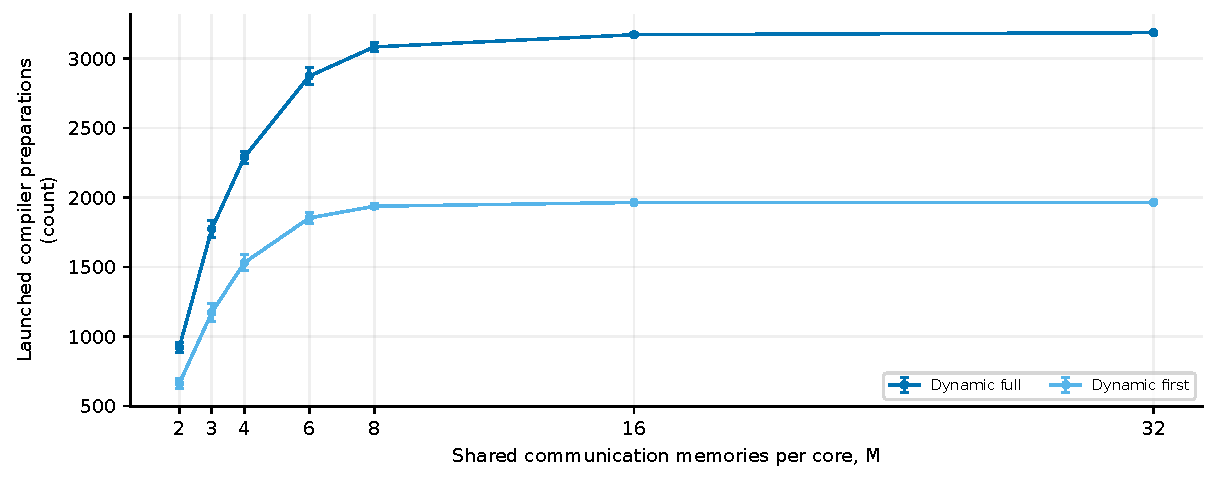
\includegraphics[width=.94\linewidth,height=.255\textheight,keepaspectratio]{figures/memory/torus_dijkstra_runtime_launched_preparations.pdf}\captionof{figure}{Run-level mean and sample SD. Shared trace aliases are counted once.}\end{center}
\begin{center}{\scriptsize\setlength{\tabcolsep}{3pt}
\begin{tabular}{lrrrrr}
\toprule
M & ODG & CGP & ACGP & Dynamic full & Dynamic first \\
\midrule
2 & n/a & n/a & n/a & $921.83\pm36.65$ & $662.00\pm37.94$ \\
3 & n/a & n/a & n/a & $1773.67\pm59.89$ & $1172.33\pm63.16$ \\
4 & n/a & n/a & n/a & $2288.00\pm44.57$ & $1529.83\pm58.47$ \\
6 & n/a & n/a & n/a & $2872.33\pm59.85$ & $1852.33\pm38.70$ \\
8 & n/a & n/a & n/a & $3082.50\pm32.20$ & $1936.50\pm18.74$ \\
16 & n/a & n/a & n/a & $3170.17\pm5.12$ & $1963.83\pm2.86$ \\
32 & n/a & n/a & n/a & $3185.00\pm2.45$ & $1965.00\pm0.00$ \\
\bottomrule\end{tabular}}
\captionof{table}{Mean $\pm$ sample SD; n/a denotes a metric outside that policy's instrumentation.}
{\footnotesize\href{https://github.com/sanjeevkrishnaa/Compiler-Driven-ACE/blob/codex/ace-scheduler-correctness/docs/latex/qft96_final/data/memory_torus_dijkstra_runtime_launched_preparations.csv}{Exact CSV values and sample counts}}
\end{center}
\subsection*{Accepted compiler preparations}
\begin{center}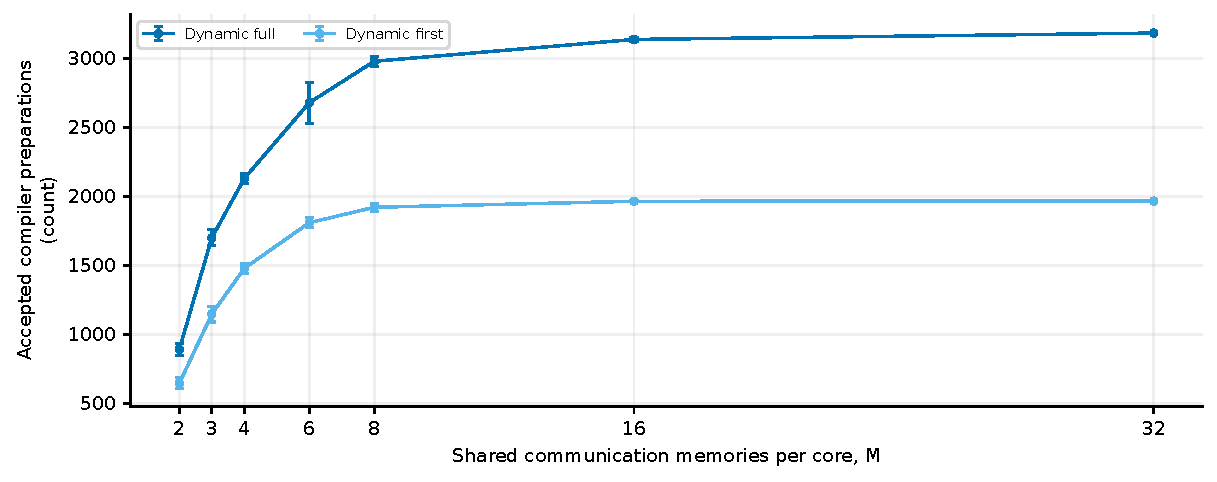
\includegraphics[width=.94\linewidth,height=.255\textheight,keepaspectratio]{figures/memory/torus_dijkstra_runtime_accepted_preparations.pdf}\captionof{figure}{Run-level mean and sample SD. Shared trace aliases are counted once.}\end{center}
\begin{center}{\scriptsize\setlength{\tabcolsep}{3pt}
\begin{tabular}{lrrrrr}
\toprule
M & ODG & CGP & ACGP & Dynamic full & Dynamic first \\
\midrule
2 & n/a & n/a & n/a & $889.83\pm44.60$ & $644.00\pm39.30$ \\
3 & n/a & n/a & n/a & $1698.83\pm56.88$ & $1145.83\pm57.26$ \\
4 & n/a & n/a & n/a & $2129.00\pm33.43$ & $1477.17\pm38.10$ \\
6 & n/a & n/a & n/a & $2678.00\pm147.34$ & $1808.00\pm37.33$ \\
8 & n/a & n/a & n/a & $2978.17\pm36.64$ & $1920.00\pm28.54$ \\
16 & n/a & n/a & n/a & $3136.67\pm11.48$ & $1963.67\pm3.27$ \\
32 & n/a & n/a & n/a & $3183.00\pm5.29$ & $1965.00\pm0.00$ \\
\bottomrule\end{tabular}}
\captionof{table}{Mean $\pm$ sample SD; n/a denotes a metric outside that policy's instrumentation.}
{\footnotesize\href{https://github.com/sanjeevkrishnaa/Compiler-Driven-ACE/blob/codex/ace-scheduler-correctness/docs/latex/qft96_final/data/memory_torus_dijkstra_runtime_accepted_preparations.csv}{Exact CSV values and sample counts}}
\end{center}
\clearpage
\subsection*{Rejected compiler preparations}
\begin{center}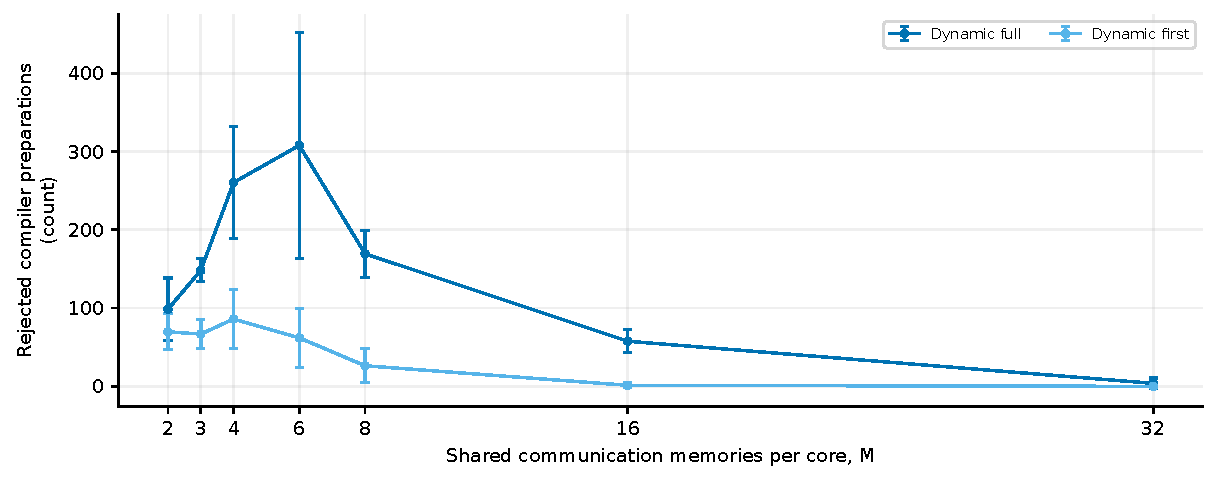
\includegraphics[width=.94\linewidth,height=.255\textheight,keepaspectratio]{figures/memory/torus_dijkstra_runtime_rejected_preparations.pdf}\captionof{figure}{Run-level mean and sample SD. Shared trace aliases are counted once.}\end{center}
\begin{center}{\scriptsize\setlength{\tabcolsep}{3pt}
\begin{tabular}{lrrrrr}
\toprule
M & ODG & CGP & ACGP & Dynamic full & Dynamic first \\
\midrule
2 & n/a & n/a & n/a & $98.500\pm39.934$ & $69.667\pm23.157$ \\
3 & n/a & n/a & n/a & $148.17\pm14.74$ & $66.833\pm18.734$ \\
4 & n/a & n/a & n/a & $260.50\pm72.02$ & $86.000\pm37.358$ \\
6 & n/a & n/a & n/a & $307.83\pm144.49$ & $62.000\pm37.968$ \\
8 & n/a & n/a & n/a & $169.50\pm30.02$ & $26.333\pm21.915$ \\
16 & n/a & n/a & n/a & $57.667\pm14.882$ & $1.333\pm3.266$ \\
32 & n/a & n/a & n/a & $3.833\pm6.882$ & $0.0000\pm0.0000$ \\
\bottomrule\end{tabular}}
\captionof{table}{Mean $\pm$ sample SD; n/a denotes a metric outside that policy's instrumentation.}
{\footnotesize\href{https://github.com/sanjeevkrishnaa/Compiler-Driven-ACE/blob/codex/ace-scheduler-correctness/docs/latex/qft96_final/data/memory_torus_dijkstra_runtime_rejected_preparations.csv}{Exact CSV values and sample counts}}
\end{center}
\subsection*{Compiler-ready request count}
\begin{center}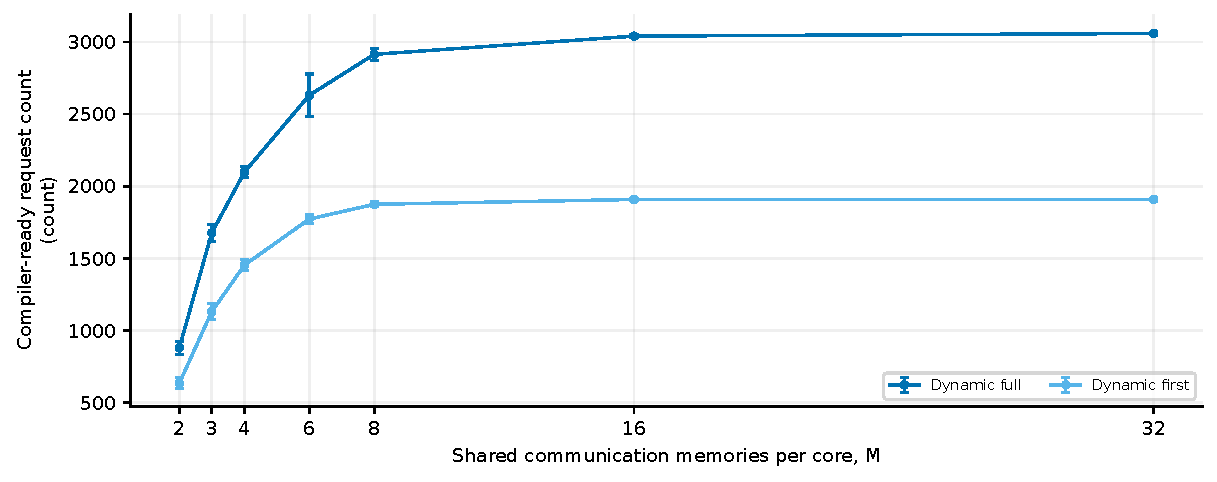
\includegraphics[width=.94\linewidth,height=.255\textheight,keepaspectratio]{figures/memory/torus_dijkstra_pregenerated_hits.pdf}\captionof{figure}{Run-level mean and sample SD. Shared trace aliases are counted once.}\end{center}
\begin{center}{\scriptsize\setlength{\tabcolsep}{3pt}
\begin{tabular}{lrrrrr}
\toprule
M & ODG & CGP & ACGP & Dynamic full & Dynamic first \\
\midrule
2 & n/a & n/a & n/a & $881.17\pm43.91$ & $636.17\pm38.72$ \\
3 & n/a & n/a & n/a & $1677.83\pm58.49$ & $1132.00\pm57.16$ \\
4 & n/a & n/a & n/a & $2096.67\pm38.32$ & $1453.33\pm36.83$ \\
6 & n/a & n/a & n/a & $2631.00\pm147.33$ & $1773.00\pm29.91$ \\
8 & n/a & n/a & n/a & $2914.50\pm39.54$ & $1875.33\pm18.15$ \\
16 & n/a & n/a & n/a & $3040.67\pm10.15$ & $1909.00\pm5.51$ \\
32 & n/a & n/a & n/a & $3059.17\pm7.86$ & $1909.50\pm5.54$ \\
\bottomrule\end{tabular}}
\captionof{table}{Mean $\pm$ sample SD; n/a denotes a metric outside that policy's instrumentation.}
{\footnotesize\href{https://github.com/sanjeevkrishnaa/Compiler-Driven-ACE/blob/codex/ace-scheduler-correctness/docs/latex/qft96_final/data/memory_torus_dijkstra_pregenerated_hits.csv}{Exact CSV values and sample counts}}
\end{center}
\clearpage
\subsection*{Intended compiler-hit count}
\begin{center}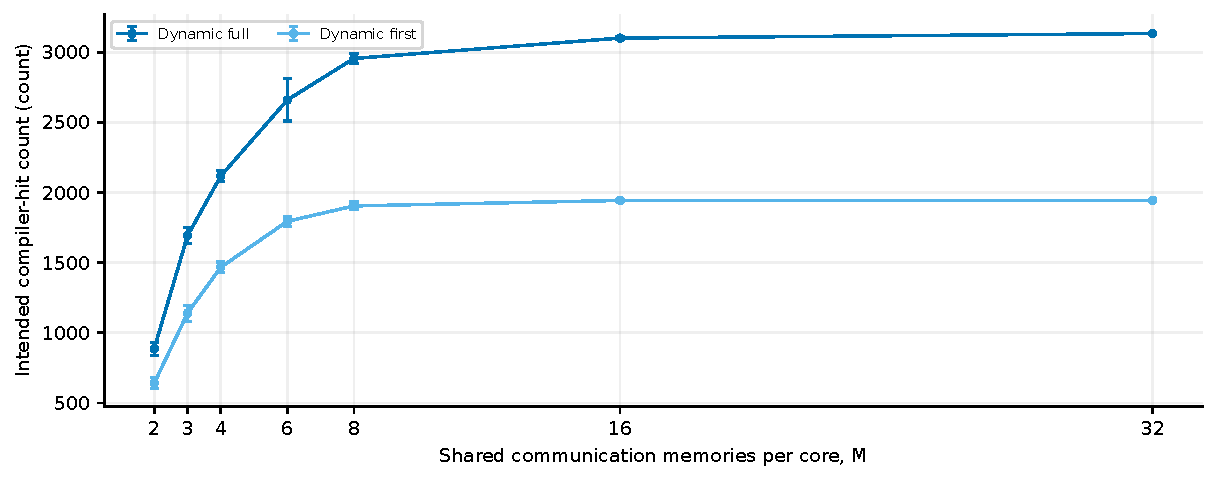
\includegraphics[width=.94\linewidth,height=.255\textheight,keepaspectratio]{figures/memory/torus_dijkstra_intended_request_hits.pdf}\captionof{figure}{Run-level mean and sample SD. Shared trace aliases are counted once.}\end{center}
\begin{center}{\scriptsize\setlength{\tabcolsep}{3pt}
\begin{tabular}{lrrrrr}
\toprule
M & ODG & CGP & ACGP & Dynamic full & Dynamic first \\
\midrule
2 & n/a & n/a & n/a & $886.50\pm45.57$ & $641.00\pm39.98$ \\
3 & n/a & n/a & n/a & $1692.67\pm57.41$ & $1139.83\pm57.23$ \\
4 & n/a & n/a & n/a & $2117.50\pm36.29$ & $1467.33\pm37.22$ \\
6 & n/a & n/a & n/a & $2660.00\pm150.13$ & $1794.50\pm36.09$ \\
8 & n/a & n/a & n/a & $2955.67\pm35.06$ & $1904.33\pm27.74$ \\
16 & n/a & n/a & n/a & $3100.83\pm12.02$ & $1943.33\pm3.93$ \\
32 & n/a & n/a & n/a & $3133.50\pm8.41$ & $1944.67\pm2.42$ \\
\bottomrule\end{tabular}}
\captionof{table}{Mean $\pm$ sample SD; n/a denotes a metric outside that policy's instrumentation.}
{\footnotesize\href{https://github.com/sanjeevkrishnaa/Compiler-Driven-ACE/blob/codex/ace-scheduler-correctness/docs/latex/qft96_final/data/memory_torus_dijkstra_intended_request_hits.csv}{Exact CSV values and sample counts}}
\end{center}
\subsection*{Compiler-not-ready request count}
\begin{center}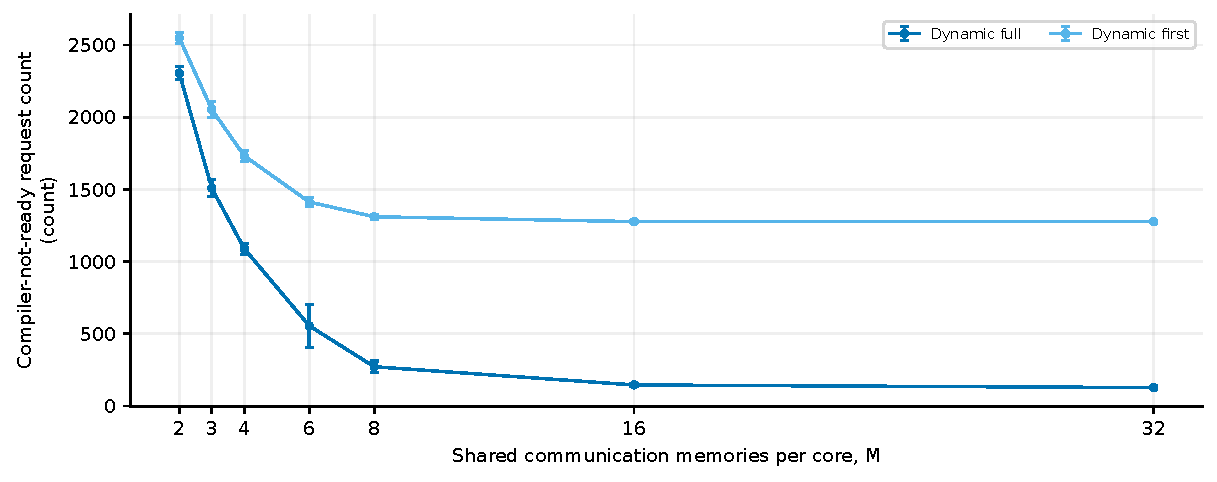
\includegraphics[width=.94\linewidth,height=.255\textheight,keepaspectratio]{figures/memory/torus_dijkstra_compiler_not_ready_requests.pdf}\captionof{figure}{Run-level mean and sample SD. Shared trace aliases are counted once.}\end{center}
\begin{center}{\scriptsize\setlength{\tabcolsep}{3pt}
\begin{tabular}{lrrrrr}
\toprule
M & ODG & CGP & ACGP & Dynamic full & Dynamic first \\
\midrule
2 & n/a & n/a & n/a & $2304.83\pm43.91$ & $2549.83\pm38.72$ \\
3 & n/a & n/a & n/a & $1508.17\pm58.49$ & $2054.00\pm57.16$ \\
4 & n/a & n/a & n/a & $1089.33\pm38.32$ & $1732.67\pm36.83$ \\
6 & n/a & n/a & n/a & $555.00\pm147.33$ & $1413.00\pm29.91$ \\
8 & n/a & n/a & n/a & $271.50\pm39.54$ & $1310.67\pm18.15$ \\
16 & n/a & n/a & n/a & $145.33\pm10.15$ & $1277.00\pm5.51$ \\
32 & n/a & n/a & n/a & $126.83\pm7.86$ & $1276.50\pm5.54$ \\
\bottomrule\end{tabular}}
\captionof{table}{Mean $\pm$ sample SD; n/a denotes a metric outside that policy's instrumentation.}
{\footnotesize\href{https://github.com/sanjeevkrishnaa/Compiler-Driven-ACE/blob/codex/ace-scheduler-correctness/docs/latex/qft96_final/data/memory_torus_dijkstra_compiler_not_ready_requests.csv}{Exact CSV values and sample counts}}
\end{center}
\clearpage
\subsection*{Late compiler-pair uses}
\begin{center}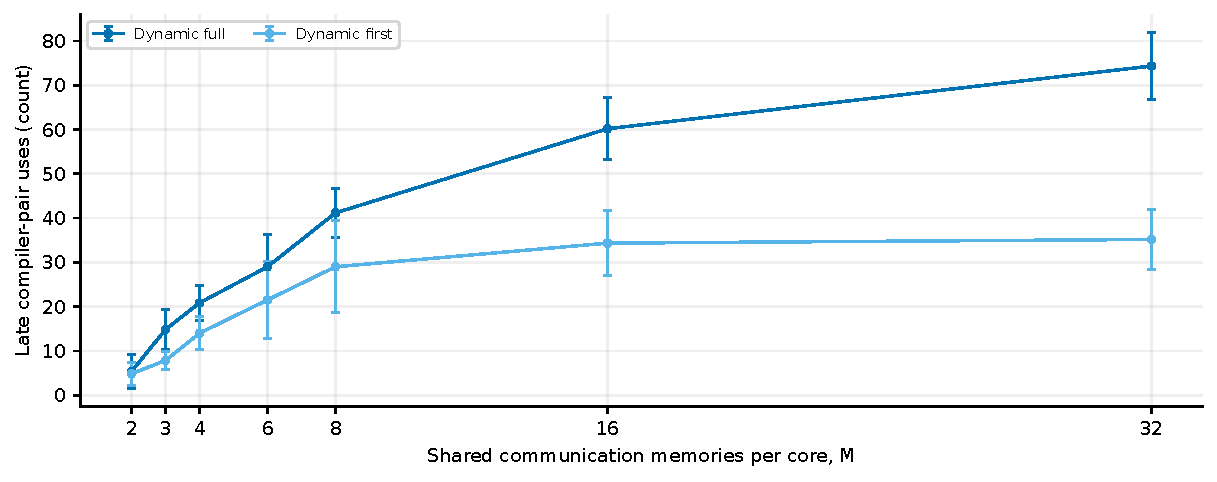
\includegraphics[width=.94\linewidth,height=.255\textheight,keepaspectratio]{figures/memory/torus_dijkstra_late_compiler_pair_uses.pdf}\captionof{figure}{Run-level mean and sample SD. Shared trace aliases are counted once.}\end{center}
\begin{center}{\scriptsize\setlength{\tabcolsep}{3pt}
\begin{tabular}{lrrrrr}
\toprule
M & ODG & CGP & ACGP & Dynamic full & Dynamic first \\
\midrule
2 & n/a & n/a & n/a & $5.333\pm3.882$ & $4.833\pm2.639$ \\
3 & n/a & n/a & n/a & $14.833\pm4.491$ & $7.833\pm1.941$ \\
4 & n/a & n/a & n/a & $20.833\pm3.971$ & $14.000\pm3.742$ \\
6 & n/a & n/a & n/a & $29.000\pm7.183$ & $21.500\pm8.643$ \\
8 & n/a & n/a & n/a & $41.167\pm5.492$ & $29.000\pm10.431$ \\
16 & n/a & n/a & n/a & $60.167\pm6.998$ & $34.333\pm7.312$ \\
32 & n/a & n/a & n/a & $74.333\pm7.607$ & $35.167\pm6.853$ \\
\bottomrule\end{tabular}}
\captionof{table}{Mean $\pm$ sample SD; n/a denotes a metric outside that policy's instrumentation.}
{\footnotesize\href{https://github.com/sanjeevkrishnaa/Compiler-Driven-ACE/blob/codex/ace-scheduler-correctness/docs/latex/qft96_final/data/memory_torus_dijkstra_late_compiler_pair_uses.csv}{Exact CSV values and sample counts}}
\end{center}
\subsection*{Compiler fallback count}
\begin{center}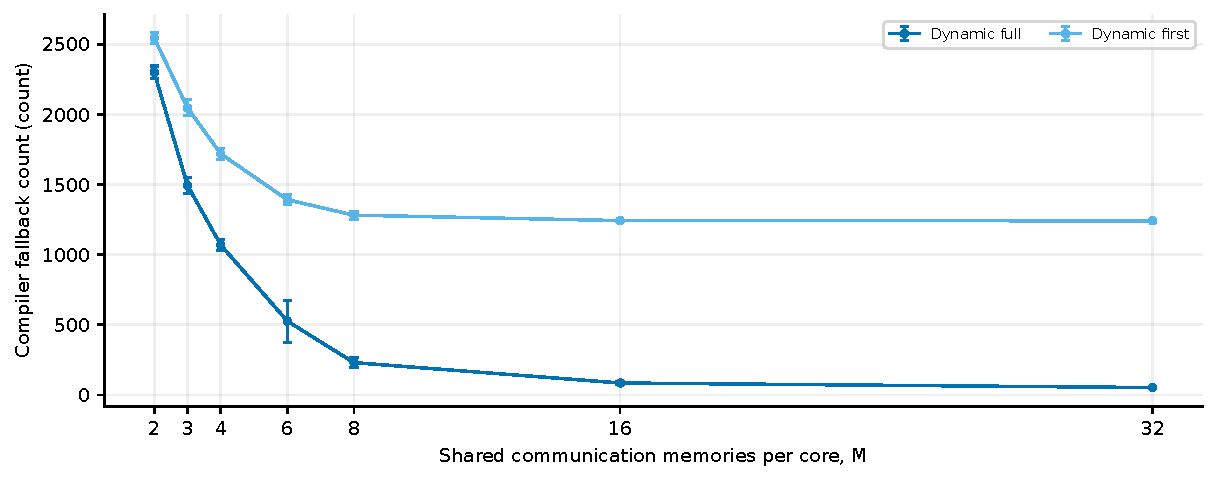
\includegraphics[width=.94\linewidth,height=.255\textheight,keepaspectratio]{figures/memory/torus_dijkstra_on_demand_fallbacks.pdf}\captionof{figure}{Run-level mean and sample SD. Shared trace aliases are counted once.}\end{center}
\begin{center}{\scriptsize\setlength{\tabcolsep}{3pt}
\begin{tabular}{lrrrrr}
\toprule
M & ODG & CGP & ACGP & Dynamic full & Dynamic first \\
\midrule
2 & n/a & n/a & n/a & $2299.50\pm45.57$ & $2545.00\pm39.98$ \\
3 & n/a & n/a & n/a & $1493.33\pm57.41$ & $2046.17\pm57.23$ \\
4 & n/a & n/a & n/a & $1068.50\pm36.29$ & $1718.67\pm37.22$ \\
6 & n/a & n/a & n/a & $526.00\pm150.13$ & $1391.50\pm36.09$ \\
8 & n/a & n/a & n/a & $230.33\pm35.06$ & $1281.67\pm27.74$ \\
16 & n/a & n/a & n/a & $85.167\pm12.024$ & $1242.67\pm3.93$ \\
32 & n/a & n/a & n/a & $52.500\pm8.408$ & $1241.33\pm2.42$ \\
\bottomrule\end{tabular}}
\captionof{table}{Mean $\pm$ sample SD; n/a denotes a metric outside that policy's instrumentation.}
{\footnotesize\href{https://github.com/sanjeevkrishnaa/Compiler-Driven-ACE/blob/codex/ace-scheduler-correctness/docs/latex/qft96_final/data/memory_torus_dijkstra_on_demand_fallbacks.csv}{Exact CSV values and sample counts}}
\end{center}
\clearpage
\subsection*{Generated compiler pairs}
\begin{center}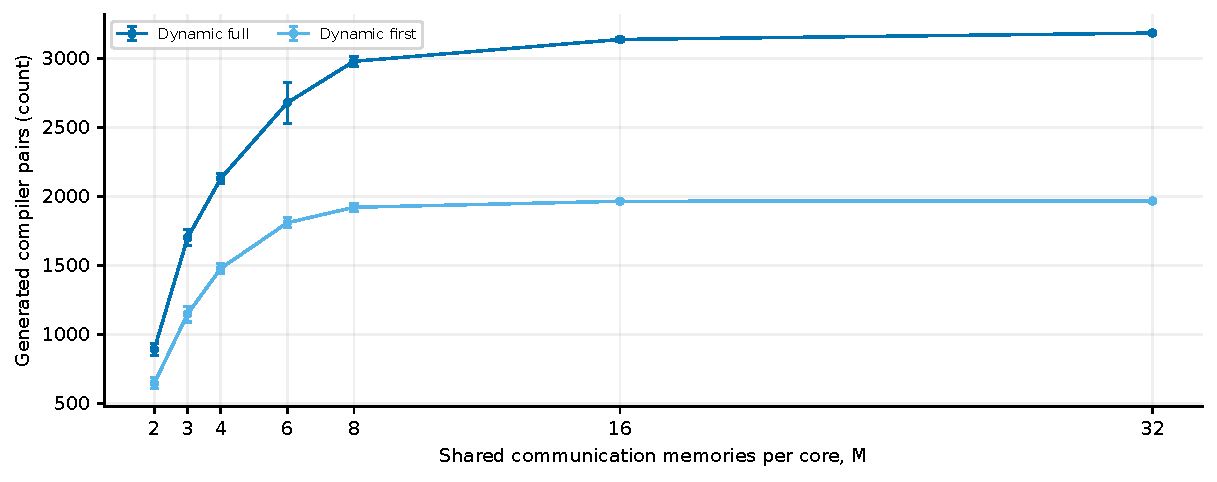
\includegraphics[width=.94\linewidth,height=.255\textheight,keepaspectratio]{figures/memory/torus_dijkstra_generated_compiler_pairs.pdf}\captionof{figure}{Run-level mean and sample SD. Shared trace aliases are counted once.}\end{center}
\begin{center}{\scriptsize\setlength{\tabcolsep}{3pt}
\begin{tabular}{lrrrrr}
\toprule
M & ODG & CGP & ACGP & Dynamic full & Dynamic first \\
\midrule
2 & n/a & n/a & n/a & $889.83\pm44.60$ & $644.00\pm39.30$ \\
3 & n/a & n/a & n/a & $1698.83\pm56.88$ & $1145.83\pm57.26$ \\
4 & n/a & n/a & n/a & $2129.00\pm33.43$ & $1477.17\pm38.10$ \\
6 & n/a & n/a & n/a & $2678.00\pm147.34$ & $1808.00\pm37.33$ \\
8 & n/a & n/a & n/a & $2978.17\pm36.64$ & $1920.00\pm28.54$ \\
16 & n/a & n/a & n/a & $3136.67\pm11.48$ & $1963.67\pm3.27$ \\
32 & n/a & n/a & n/a & $3183.00\pm5.29$ & $1965.00\pm0.00$ \\
\bottomrule\end{tabular}}
\captionof{table}{Mean $\pm$ sample SD; n/a denotes a metric outside that policy's instrumentation.}
{\footnotesize\href{https://github.com/sanjeevkrishnaa/Compiler-Driven-ACE/blob/codex/ace-scheduler-correctness/docs/latex/qft96_final/data/memory_torus_dijkstra_generated_compiler_pairs.csv}{Exact CSV values and sample counts}}
\end{center}
\subsection*{Used compiler pairs}
\begin{center}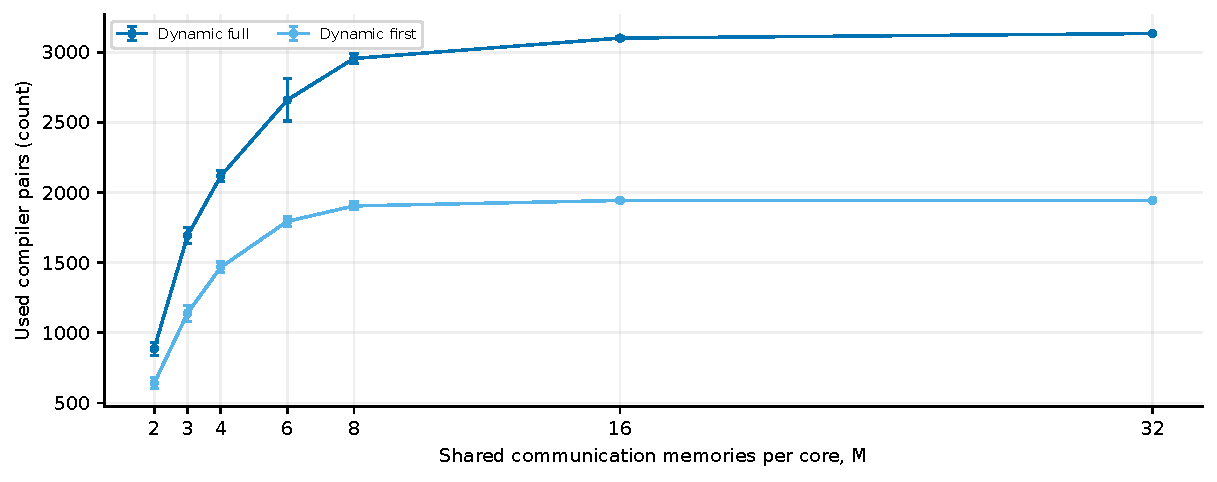
\includegraphics[width=.94\linewidth,height=.255\textheight,keepaspectratio]{figures/memory/torus_dijkstra_utilized_compiler_pairs.pdf}\captionof{figure}{Run-level mean and sample SD. Shared trace aliases are counted once.}\end{center}
\begin{center}{\scriptsize\setlength{\tabcolsep}{3pt}
\begin{tabular}{lrrrrr}
\toprule
M & ODG & CGP & ACGP & Dynamic full & Dynamic first \\
\midrule
2 & n/a & n/a & n/a & $886.50\pm45.57$ & $641.00\pm39.98$ \\
3 & n/a & n/a & n/a & $1692.67\pm57.41$ & $1139.83\pm57.23$ \\
4 & n/a & n/a & n/a & $2117.50\pm36.29$ & $1467.33\pm37.22$ \\
6 & n/a & n/a & n/a & $2660.00\pm150.13$ & $1794.50\pm36.09$ \\
8 & n/a & n/a & n/a & $2955.67\pm35.06$ & $1904.33\pm27.74$ \\
16 & n/a & n/a & n/a & $3100.83\pm12.02$ & $1943.33\pm3.93$ \\
32 & n/a & n/a & n/a & $3133.50\pm8.41$ & $1944.67\pm2.42$ \\
\bottomrule\end{tabular}}
\captionof{table}{Mean $\pm$ sample SD; n/a denotes a metric outside that policy's instrumentation.}
{\footnotesize\href{https://github.com/sanjeevkrishnaa/Compiler-Driven-ACE/blob/codex/ace-scheduler-correctness/docs/latex/qft96_final/data/memory_torus_dijkstra_utilized_compiler_pairs.csv}{Exact CSV values and sample counts}}
\end{center}
\clearpage
\subsection*{Expired compiler pairs}
\begin{center}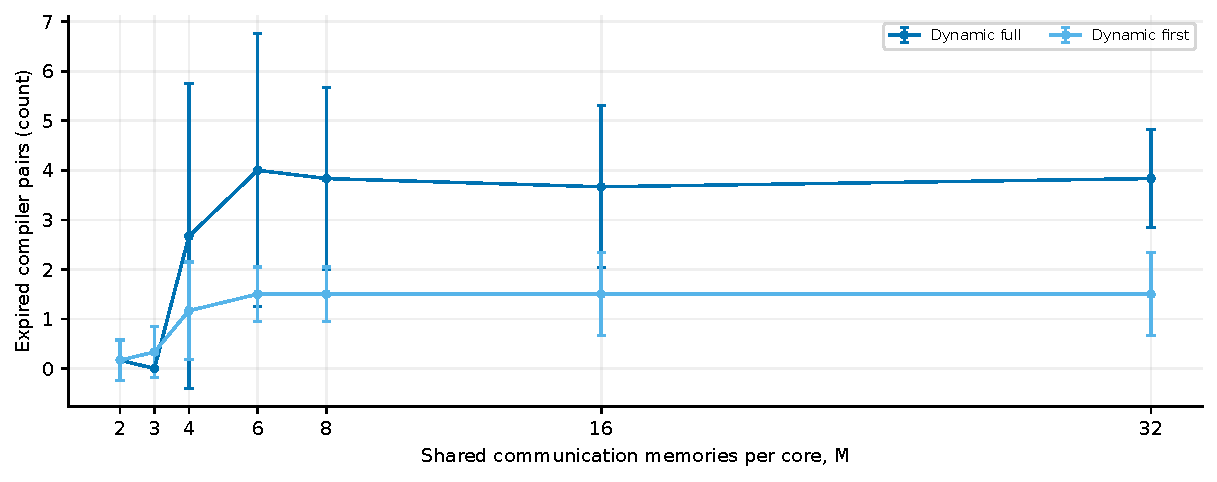
\includegraphics[width=.94\linewidth,height=.255\textheight,keepaspectratio]{figures/memory/torus_dijkstra_expired_compiler_pairs.pdf}\captionof{figure}{Run-level mean and sample SD. Shared trace aliases are counted once.}\end{center}
\begin{center}{\scriptsize\setlength{\tabcolsep}{3pt}
\begin{tabular}{lrrrrr}
\toprule
M & ODG & CGP & ACGP & Dynamic full & Dynamic first \\
\midrule
2 & n/a & n/a & n/a & $0.1667\pm0.4082$ & $0.1667\pm0.4082$ \\
3 & n/a & n/a & n/a & $0.0000\pm0.0000$ & $0.3333\pm0.5164$ \\
4 & n/a & n/a & n/a & $2.667\pm3.077$ & $1.167\pm0.983$ \\
6 & n/a & n/a & n/a & $4.000\pm2.757$ & $1.500\pm0.548$ \\
8 & n/a & n/a & n/a & $3.833\pm1.835$ & $1.500\pm0.548$ \\
16 & n/a & n/a & n/a & $3.667\pm1.633$ & $1.500\pm0.837$ \\
32 & n/a & n/a & n/a & $3.833\pm0.983$ & $1.500\pm0.837$ \\
\bottomrule\end{tabular}}
\captionof{table}{Mean $\pm$ sample SD; n/a denotes a metric outside that policy's instrumentation.}
{\footnotesize\href{https://github.com/sanjeevkrishnaa/Compiler-Driven-ACE/blob/codex/ace-scheduler-correctness/docs/latex/qft96_final/data/memory_torus_dijkstra_expired_compiler_pairs.csv}{Exact CSV values and sample counts}}
\end{center}
\subsection*{Remaining compiler pairs}
\begin{center}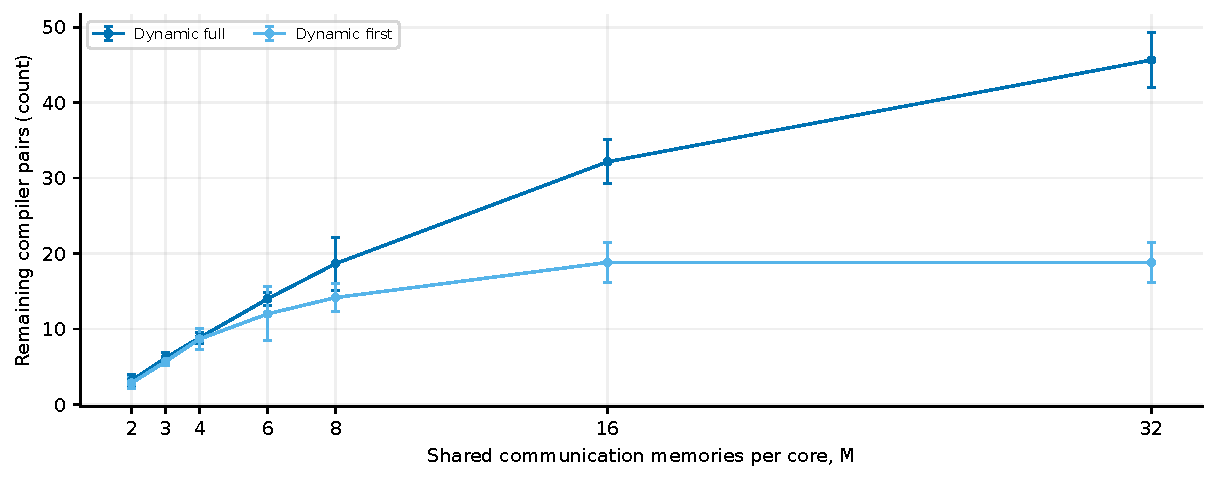
\includegraphics[width=.94\linewidth,height=.255\textheight,keepaspectratio]{figures/memory/torus_dijkstra_remaining_compiler_pairs.pdf}\captionof{figure}{Run-level mean and sample SD. Shared trace aliases are counted once.}\end{center}
\begin{center}{\scriptsize\setlength{\tabcolsep}{3pt}
\begin{tabular}{lrrrrr}
\toprule
M & ODG & CGP & ACGP & Dynamic full & Dynamic first \\
\midrule
2 & n/a & n/a & n/a & $3.167\pm0.753$ & $2.833\pm0.753$ \\
3 & n/a & n/a & n/a & $6.167\pm0.753$ & $5.667\pm0.516$ \\
4 & n/a & n/a & n/a & $8.833\pm0.753$ & $8.667\pm1.366$ \\
6 & n/a & n/a & n/a & $14.000\pm0.894$ & $12.000\pm3.578$ \\
8 & n/a & n/a & n/a & $18.667\pm3.502$ & $14.167\pm1.835$ \\
16 & n/a & n/a & n/a & $32.167\pm2.927$ & $18.833\pm2.639$ \\
32 & n/a & n/a & n/a & $45.667\pm3.670$ & $18.833\pm2.639$ \\
\bottomrule\end{tabular}}
\captionof{table}{Mean $\pm$ sample SD; n/a denotes a metric outside that policy's instrumentation.}
{\footnotesize\href{https://github.com/sanjeevkrishnaa/Compiler-Driven-ACE/blob/codex/ace-scheduler-correctness/docs/latex/qft96_final/data/memory_torus_dijkstra_remaining_compiler_pairs.csv}{Exact CSV values and sample counts}}
\end{center}
\clearpage
\subsection*{Compiler fidelity at creation}
\begin{center}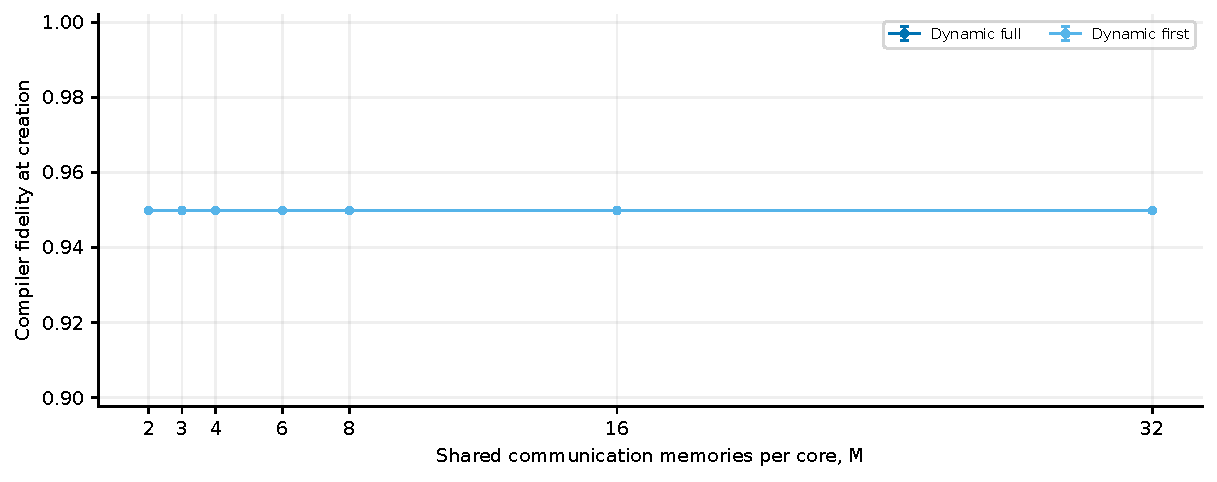
\includegraphics[width=.94\linewidth,height=.255\textheight,keepaspectratio]{figures/memory/torus_dijkstra_average_fidelity_at_creation.pdf}\captionof{figure}{Run-level mean and sample SD. Shared trace aliases are counted once.}\end{center}
\begin{center}{\scriptsize\setlength{\tabcolsep}{3pt}
\begin{tabular}{lrrrrr}
\toprule
M & ODG & CGP & ACGP & Dynamic full & Dynamic first \\
\midrule
2 & n/a & n/a & n/a & $0.9498\pm0.0000$ & $0.9498\pm0.0000$ \\
3 & n/a & n/a & n/a & $0.9498\pm0.0000$ & $0.9498\pm0.0000$ \\
4 & n/a & n/a & n/a & $0.9498\pm0.0000$ & $0.9498\pm0.0000$ \\
6 & n/a & n/a & n/a & $0.9498\pm0.0000$ & $0.9498\pm0.0000$ \\
8 & n/a & n/a & n/a & $0.9498\pm0.0000$ & $0.9498\pm0.0000$ \\
16 & n/a & n/a & n/a & $0.9498\pm0.0000$ & $0.9498\pm0.0000$ \\
32 & n/a & n/a & n/a & $0.9498\pm0.0000$ & $0.9498\pm0.0000$ \\
\bottomrule\end{tabular}}
\captionof{table}{Mean $\pm$ sample SD; n/a denotes a metric outside that policy's instrumentation.}
{\footnotesize\href{https://github.com/sanjeevkrishnaa/Compiler-Driven-ACE/blob/codex/ace-scheduler-correctness/docs/latex/qft96_final/data/memory_torus_dijkstra_average_fidelity_at_creation.csv}{Exact CSV values and sample counts}}
\end{center}
\subsection*{Compiler fidelity at use}
\begin{center}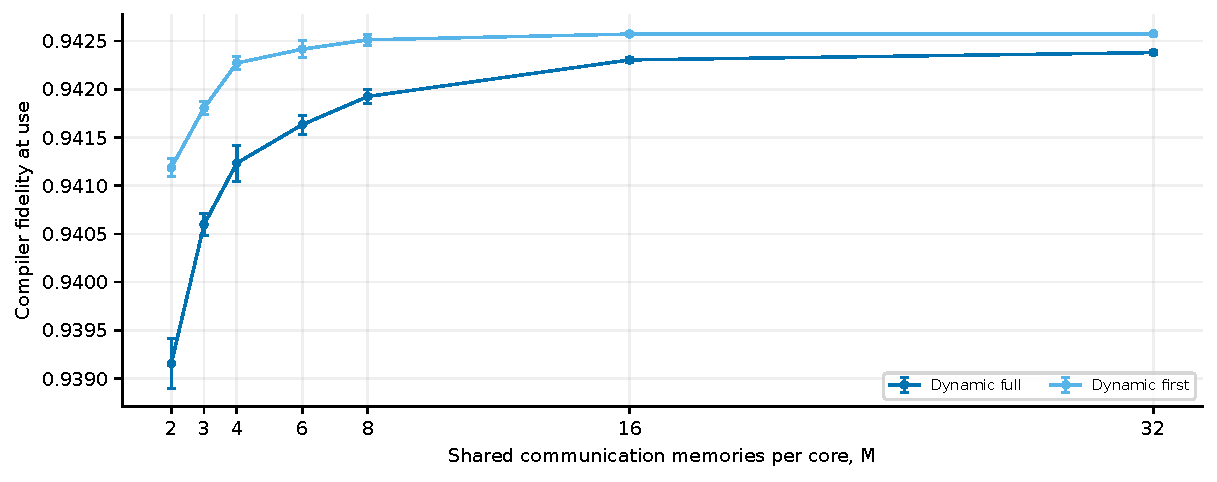
\includegraphics[width=.94\linewidth,height=.255\textheight,keepaspectratio]{figures/memory/torus_dijkstra_average_fidelity_at_utilization.pdf}\captionof{figure}{Run-level mean and sample SD. Shared trace aliases are counted once.}\end{center}
\begin{center}{\scriptsize\setlength{\tabcolsep}{3pt}
\begin{tabular}{lrrrrr}
\toprule
M & ODG & CGP & ACGP & Dynamic full & Dynamic first \\
\midrule
2 & n/a & n/a & n/a & $0.9392\pm0.0003$ & $0.9412\pm0.0001$ \\
3 & n/a & n/a & n/a & $0.9406\pm0.0001$ & $0.9418\pm0.0001$ \\
4 & n/a & n/a & n/a & $0.9412\pm0.0002$ & $0.9423\pm0.0001$ \\
6 & n/a & n/a & n/a & $0.9416\pm0.0001$ & $0.9424\pm0.0001$ \\
8 & n/a & n/a & n/a & $0.9419\pm0.0001$ & $0.9425\pm0.0001$ \\
16 & n/a & n/a & n/a & $0.9423\pm0.0000$ & $0.9426\pm0.0000$ \\
32 & n/a & n/a & n/a & $0.9424\pm0.0000$ & $0.9426\pm0.0000$ \\
\bottomrule\end{tabular}}
\captionof{table}{Mean $\pm$ sample SD; n/a denotes a metric outside that policy's instrumentation.}
{\footnotesize\href{https://github.com/sanjeevkrishnaa/Compiler-Driven-ACE/blob/codex/ace-scheduler-correctness/docs/latex/qft96_final/data/memory_torus_dijkstra_average_fidelity_at_utilization.csv}{Exact CSV values and sample counts}}
\end{center}
\clearpage
\subsection*{Mean layer latency}
\begin{center}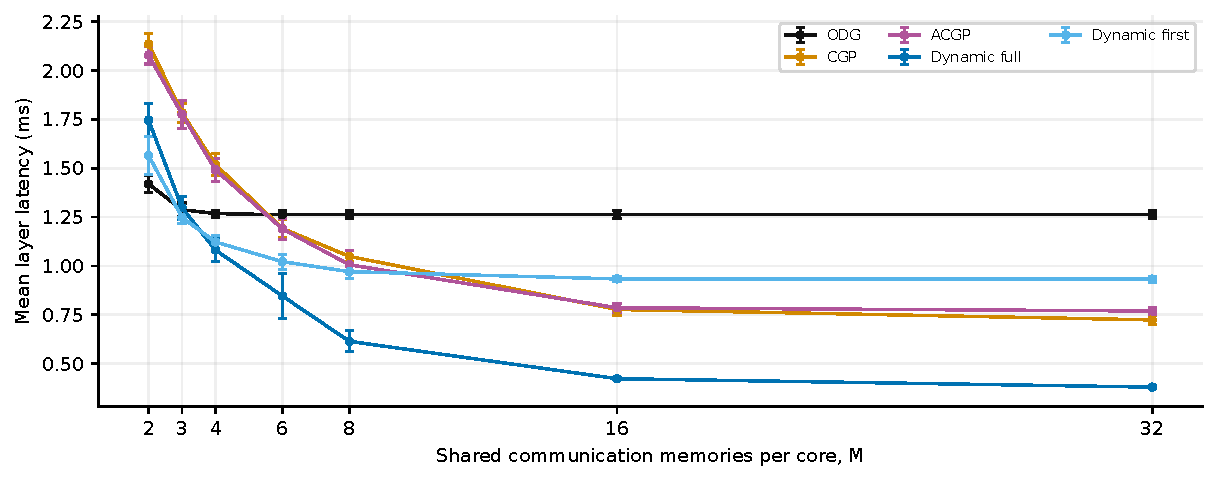
\includegraphics[width=.94\linewidth,height=.255\textheight,keepaspectratio]{figures/memory/torus_dijkstra_avg_layer_latency_ms.pdf}\captionof{figure}{Run-level mean and sample SD. Shared trace aliases are counted once.}\end{center}
\begin{center}{\scriptsize\setlength{\tabcolsep}{3pt}
\begin{tabular}{lrrrrr}
\toprule
M & ODG & CGP & ACGP & Dynamic full & Dynamic first \\
\midrule
2 & $1.419\pm0.043$ & $2.135\pm0.053$ & $2.079\pm0.045$ & $1.746\pm0.084$ & $1.565\pm0.095$ \\
3 & $1.288\pm0.034$ & $1.783\pm0.050$ & $1.776\pm0.072$ & $1.298\pm0.059$ & $1.248\pm0.033$ \\
4 & $1.268\pm0.018$ & $1.518\pm0.055$ & $1.492\pm0.060$ & $1.081\pm0.059$ & $1.122\pm0.033$ \\
6 & $1.262\pm0.021$ & $1.192\pm0.047$ & $1.189\pm0.054$ & $0.8462\pm0.1154$ & $1.022\pm0.039$ \\
8 & $1.263\pm0.021$ & $1.049\pm0.029$ & $1.006\pm0.072$ & $0.6142\pm0.0542$ & $0.9706\pm0.0360$ \\
16 & $1.263\pm0.021$ & $0.7771\pm0.0284$ & $0.7860\pm0.0217$ & $0.4230\pm0.0058$ & $0.9333\pm0.0149$ \\
32 & $1.263\pm0.021$ & $0.7237\pm0.0231$ & $0.7692\pm0.0182$ & $0.3797\pm0.0086$ & $0.9326\pm0.0149$ \\
\bottomrule\end{tabular}}
\captionof{table}{Mean $\pm$ sample SD; n/a denotes a metric outside that policy's instrumentation.}
{\footnotesize\href{https://github.com/sanjeevkrishnaa/Compiler-Driven-ACE/blob/codex/ace-scheduler-correctness/docs/latex/qft96_final/data/memory_torus_dijkstra_avg_layer_latency_ms.csv}{Exact CSV values and sample counts}}
\end{center}
\subsection*{Maximum layer latency}
\begin{center}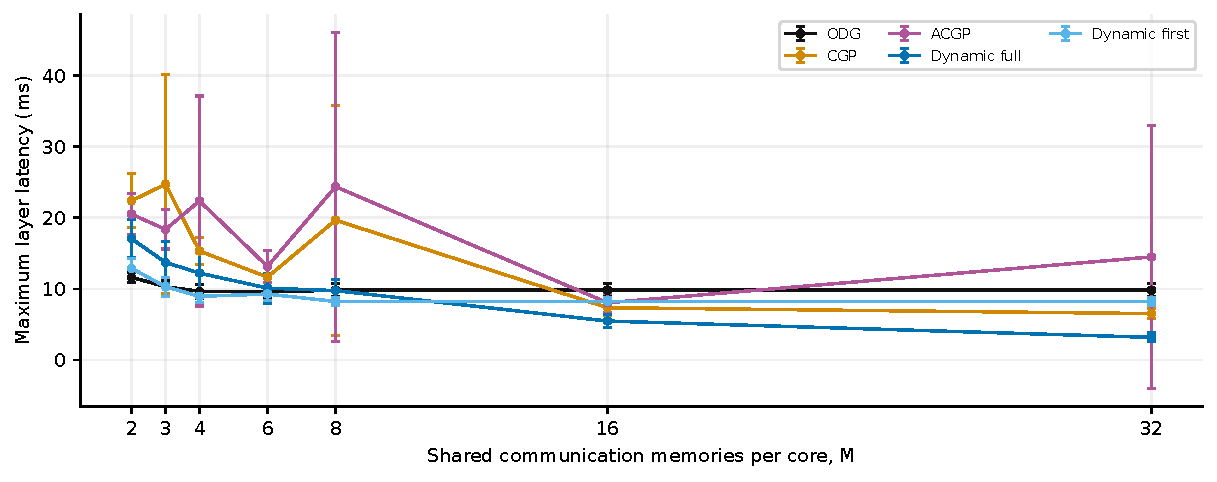
\includegraphics[width=.94\linewidth,height=.255\textheight,keepaspectratio]{figures/memory/torus_dijkstra_max_layer_latency_ms.pdf}\captionof{figure}{Run-level mean and sample SD. Shared trace aliases are counted once.}\end{center}
\begin{center}{\scriptsize\setlength{\tabcolsep}{3pt}
\begin{tabular}{lrrrrr}
\toprule
M & ODG & CGP & ACGP & Dynamic full & Dynamic first \\
\midrule
2 & $11.634\pm0.739$ & $22.401\pm3.830$ & $20.515\pm2.894$ & $17.067\pm2.692$ & $12.884\pm1.441$ \\
3 & $10.300\pm0.927$ & $24.717\pm15.411$ & $18.367\pm2.764$ & $13.717\pm2.925$ & $10.300\pm1.345$ \\
4 & $9.650\pm0.954$ & $15.317\pm1.887$ & $22.366\pm14.776$ & $12.217\pm2.865$ & $8.950\pm0.864$ \\
6 & $9.550\pm0.779$ & $11.651\pm1.485$ & $13.150\pm2.276$ & $10.100\pm2.105$ & $9.267\pm0.852$ \\
8 & $9.817\pm0.968$ & $19.667\pm16.176$ & $24.379\pm21.728$ & $9.750\pm1.615$ & $8.217\pm0.560$ \\
16 & $9.817\pm0.968$ & $7.346\pm1.045$ & $8.036\pm1.338$ & $5.467\pm0.922$ & $8.217\pm0.560$ \\
32 & $9.817\pm0.968$ & $6.517\pm0.662$ & $14.492\pm18.554$ & $3.167\pm0.615$ & $8.217\pm0.560$ \\
\bottomrule\end{tabular}}
\captionof{table}{Mean $\pm$ sample SD; n/a denotes a metric outside that policy's instrumentation.}
{\footnotesize\href{https://github.com/sanjeevkrishnaa/Compiler-Driven-ACE/blob/codex/ace-scheduler-correctness/docs/latex/qft96_final/data/memory_torus_dijkstra_max_layer_latency_ms.csv}{Exact CSV values and sample counts}}
\end{center}
\clearpage
\subsection*{Minimum layer latency}
\begin{center}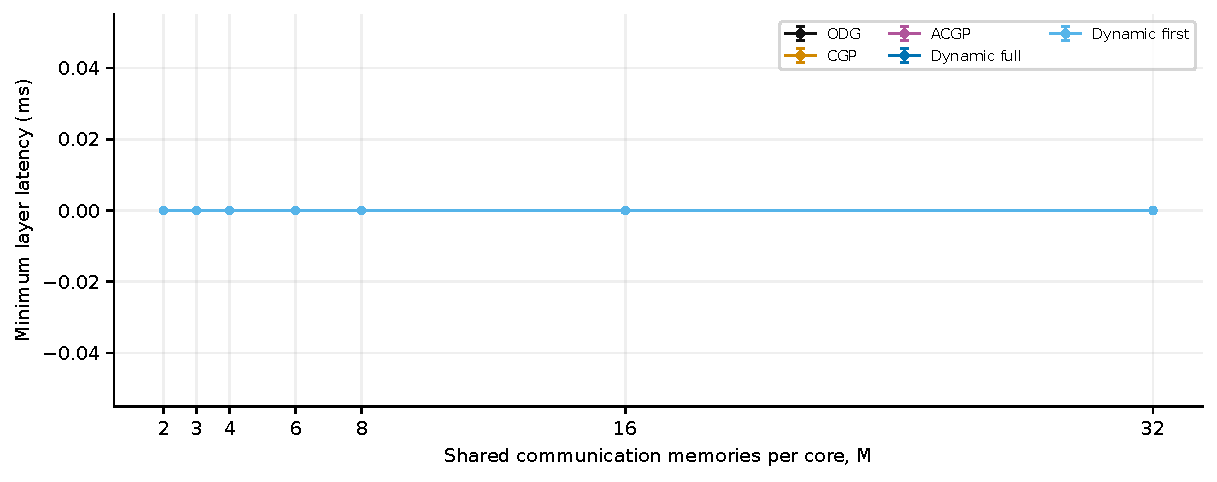
\includegraphics[width=.94\linewidth,height=.255\textheight,keepaspectratio]{figures/memory/torus_dijkstra_min_layer_latency_ms.pdf}\captionof{figure}{Run-level mean and sample SD. Shared trace aliases are counted once.}\end{center}
\begin{center}{\scriptsize\setlength{\tabcolsep}{3pt}
\begin{tabular}{lrrrrr}
\toprule
M & ODG & CGP & ACGP & Dynamic full & Dynamic first \\
\midrule
2 & $0.0000\pm0.0000$ & $0.0000\pm0.0000$ & $0.0000\pm0.0000$ & $0.0000\pm0.0000$ & $0.0000\pm0.0000$ \\
3 & $0.0000\pm0.0000$ & $0.0000\pm0.0000$ & $0.0000\pm0.0000$ & $0.0000\pm0.0000$ & $0.0000\pm0.0000$ \\
4 & $0.0000\pm0.0000$ & $0.0000\pm0.0000$ & $0.0000\pm0.0000$ & $0.0000\pm0.0000$ & $0.0000\pm0.0000$ \\
6 & $0.0000\pm0.0000$ & $0.0000\pm0.0000$ & $0.0000\pm0.0000$ & $0.0000\pm0.0000$ & $0.0000\pm0.0000$ \\
8 & $0.0000\pm0.0000$ & $0.0000\pm0.0000$ & $0.0000\pm0.0000$ & $0.0000\pm0.0000$ & $0.0000\pm0.0000$ \\
16 & $0.0000\pm0.0000$ & $0.0000\pm0.0000$ & $0.0000\pm0.0000$ & $0.0000\pm0.0000$ & $0.0000\pm0.0000$ \\
32 & $0.0000\pm0.0000$ & $0.0000\pm0.0000$ & $0.0000\pm0.0000$ & $0.0000\pm0.0000$ & $0.0000\pm0.0000$ \\
\bottomrule\end{tabular}}
\captionof{table}{Mean $\pm$ sample SD; n/a denotes a metric outside that policy's instrumentation.}
{\footnotesize\href{https://github.com/sanjeevkrishnaa/Compiler-Driven-ACE/blob/codex/ace-scheduler-correctness/docs/latex/qft96_final/data/memory_torus_dijkstra_min_layer_latency_ms.csv}{Exact CSV values and sample counts}}
\end{center}